\documentclass[german,english,twoside,headsepline,titlepage=true]{scrartcl}
% Header, der in jedem meiner Dokumente drinhängt.
% Setzt Rechtschreibung, Hyperlinks, Schriftart und Typographie

\usepackage[]{babel}
\usepackage{xparse}
\usepackage[colorlinks=true,linkcolor=blue,pdfborder={0 0 0}]{hyperref}
\usepackage{hyperxmp}
\usepackage{microtype}
%\usepackage[scale=3]{ccicons}


\usepackage{fontspec}
\setmainfont[]{Linux Libertine O}
\setsansfont{Linux Biolinum O}

\usepackage{todonotes}
\usepackage[left]{showlabels}
\input{header_math}
\input{header_artcl}


\usepackage{chemformula}
\usepackage[exponent-product = \cdot]{siunitx}
\usepackage{graphicx}
\graphicspath{ {images/} }

% \usepackage{gnuplottex}
\newfontfamily\nfrac[Fractions=On]{Linux Libertine O}
%\newfontfamily\diagram[Size=.5]{Linux Libertine O}

\usepackage{pgfplots}

\usepackage{ccicons}

\addfontfeature{Fractions=On}

% Schmutztitel
\KOMAoption{twoside}{false}
\extratitle{
  ~
  \begin{center}
    \huge \textbf{Fakultät für Physik \& Astronomie}
  \end{center}
  ~
  \begin{center}
    \Large \textbf{Ruprecht-Karls-Universität Heidelberg}
  \end{center}
  \vfill
  \begin{center}
    \Large \textbf{Bachelor-Arbeit}\\[1ex]
    im Studiengang Physik\\
    vorgelegt von \\[1ex]
    \Large \textbf{Tim Adler}\\[1ex]
    geboren in Sinsheim
  \end{center}
  ~
  \begin{center}
    \huge \textbf{2016}
  \end{center}
}

\KOMAoption{twoside}{true}

\titlehead{Universität Heidelberg \\
  Fakultät für Physik \& Astronomie\\
  Im Neuenheimer Feld 226\\
  69120 Heidelberg}
\subject{Bachelor-Arbeit}
\title{Ein Konverter}
\author{Tim Adler}
\date{\today}
\publishers{Betreut durch Dr.\ Denis Pöhler und Prof.\ Dr.\ Ulrich Platt}
\uppertitleback{Tim Adler\\Eberlinweg 6\\69121
  Heidelberg\\tim \{at\} emrys-merlin.de}
\lowertitleback{
\textbf{Ein Konverter}\\
Bachelor Thesis in the degree program Physics (B.\,Sc.)\\[\baselineskip]
Heidelberg University\\
Department for Physics and Astronomy\\
Institute for Environmental Physics\\[\baselineskip]
\begin{tabular}[htbp]{l l}
Advised by & Dr.\ Denis Pöhler, Dr.\ Martin Horbanski and Prof.\ Dr.\ Ulrich Platt\\
Starting date & 17.\ Januar 2016 \\
Closing date & \today\\
\end{tabular}
\\[\baselineskip]
\ccbysa\vspace{0.2cm}\\
This thesis is licensed under a
Creative Commons Attribution-ShareAlike 3.0 Unported License. See
\url{http://creativecommons.org/licenses/by-sa/3.0/} for more information.\\[\baselineskip]
This work has been set using {\LaTeX} and {\KOMAScript}.\\[\baselineskip]
\begin{tabular}[htbp]{r l}
  Main Font: & Linux Libertine O\\
  Sans Font: & Linux Biolinum O
\end{tabular}}

\makeatletter
\hypersetup{
  pdftitle={\@title},
  pdfauthor={\@author},
  pdfdate={\@date}
}
\makeatother

\begin{document}

\pagenumbering{roman}
\selectlanguage{german}
\maketitle
\selectlanguage{english}

\listoftodos
\todo{ToDo-Liste entfernen.}
\newpage

\selectlanguage{german}

\subsubsection*{Zusammenfassung}
\label{sec:Zusammenfassung}

Diese Bachelor-Arbeit zielt darauf ab einen
Stickstoffmonoxid-zu-Stickstoffdioxid-Konverter weiter zu
verbessern. Dieser soll zusammen mit einem CE-DOAS Messinstrument
verwendet werden, um die Stickoxid-Belastung in städtischen Gebieten
zu bestimmen. Der Hauptbestandteil dieses Konverters ist ein
Ozon-Generator. Es war uns möglich seine Luft völlig von
Stickstoffdioxid (\ch{NO2}) zu säubern, was seine Verwendung in dem
Konverter erst ermöglichte. Im Anschluß, charakterisierten wir eben
diesen und bestimmten die mögliche \ch{NO} Messgenauigkeit in
Laborsystemen. Zusätzlich testeten wir erste Anwendungen durch
Fahrzeugmessungen im Stadtgebiet Heidelberg. Es sind immer noch weiter
Untersuchungen nötig um das Potential des Konverters voll
auszuschöpfen. Insbesondere ist ein besseres Verständnis des
Adsorptionsverhaltens von Ozon an den Teflonschläuchen nötig, um
weitere pragmatischere Messmethoden zu ermöglichen.

\selectlanguage{english}

\subsubsection*{Abstract}
\label{sec:abstract}

This Bachelor Thesis aims at an further improvement of a nitrogen
monoxide (\ch{NO}) to nitrogen dioxide (\ch{NO2}) converter, which
will be used in conjunction with a CE-DOAS instrument to measure the
nitrogen oxide pollution in urban areas. The main component of this
converter is an ozone generator. We succeeded in making its output
\ch{NO2} free and thus making its use in the converter possible. We
then turn towards the characterisation of the converter and determine
the possible \ch{NO} measurement accuracy. Additionally, we tested
first productive applications by performing live vehicle measurements
in Heidelberg. There are still further investigations necessary to
reach the full potential of this setup. First and foremost the
adsorption behaviour of ozone at the teflon walls of the tubes has to
be determined in order to allow for more practical measurement modes.

%%% Local Variables: 
%%% mode: latex
%%% TeX-master: "../Bachelor"
%%% End: 

\newpage

% Nur bis section, nicht bis subsection
\setcounter{tocdepth}{2}
\tableofcontents
\cleardoubleoddstandardpage{}
\pagenumbering{arabic}
\section{Introduction}
\label{sec:intro}

This bachelor thesis stands in a row of theses all concerned with the
improvement of nitrogen oxide detection capabilities of nitrogen
dioxide CE-DOAS instruments. Nitrogen oxides (\ch{NO_x}) play an
important role in the atmospherical chemistry of urban areas
(c.\,f.~\cite{roedel}) and are major air pollutants in German cities
(c.\,f.~\cite{no2schadstoff,who}). Together with other volatile
organic compounds, they can build up ozone, leading to higher health
risks. In addition, they are toxic in their own right.

In inhabitated areas, most nitrogen oxide is anthropogenic, as it is
generated during combustion processes, e.\,g.\ in car engines. Strict
regulation and monitoring by government agencies is necessary to
protect the air quality. However, the recent VW affair shows that
there is still a lack of adequate monitoring instruments. There is a
need for mobile and reasonably priced measurement units, which can be
used to determine the \ch{NO_x} emissions under live conditions; in
the streets, during regular traffic.

A first succesful step towards such an instrument is the compact
\ch{NO2} ICAD (Iterative Cavity DOAS)
instrument developed at the Institute of Environmental Physics at
Heidelberg University. It is a further development of the CE-DOAS
technique. With a led in the blue light spectrum, it can determine
nitrogen dioxide (\ch{NO2}) concentrations with a very high accuracy,
while being portable and easily installable in vehicles for in vivo
measurements. However, there is still room for improvement. Nitrogen
monoxide (\ch{NO}) is also a central component in the atmospheric
\ch{NO_x} equilibrium, but it can only be detected in the deep
ultraviolet wavelength range. This is a dilemma as UV leds are still
expensive and highly reflective mirrors in that range are so far not
available, making such an upgrade unattractive. Luckily, there is a
workaround for this problem. There is a promising conversion from
\ch{NO} to \ch{NO2}, which would allow us to measure the concentration
indirectly. The details of this converter construction are the topic
of this work.

Zimmermann~\cite{zimmermann}, Gerick~\cite{gerick} and
Jegminat~\cite{bsc} have already established, that ambient air
together with a mercury lamp can be used to generate ozone, which in
turn triggers the desired conversion. However, there are still a few
stumbling blocks left. The ozone generator produces \ch{NO2}, too,
which disturbs the measured \ch{NO_x} signals. Jegminat found that
this additional signal is due to laughing gas (\ch{N2O}), which is
very hard to filter. Therefore, this work explores the possibilities
of filtering the \ch{NO2} behind the generator, while avoiding the
removal of the necessary ozone. Silica gel is used
as~\cite{ozone-silica} inidicates, that it will quickly be saturated
by ozone, while this work investigates if it then still may adsorb
nitrogen dioxide. This work confirmed this hypothesis and determined
the filtering efffects. After having assured a clean ozone air stream,
precisely controlled \ch{NO} concentrations within synthetic air were
used to determine the accuracy of our conversion. Afterwards, the
alternating measurement mode, which switches between \ch{NO2} and
\ch{NO}+\ch{NO2} measurements, was characterized. It was found that
necessary purge times in between measurements had to be determined to
ensure that stable equilibria were reached. This investigation found
that ozone adsorption at the teflon tubes might be a major drawback,
when it comes to quickly draining the system of it. If one measurement
mode (i.\,e. \ch{NO2} or \ch{NO_x}) is fixed, no additional adsorption
effects seem to occur. With this configuration measurements using
ambient air were performed and results were compared to a
chemiluminescence monitor. Finally, this work applied the new system
to the above mentioned vehicle measurements (within Heidelberg). The
updated ICAD instrument together with a second (pure \ch{NO2})
measurement cell was installed in a car and the plume of ca.~30
vehicles was measured. Additionally, measurements next to the
Heidelberg air quality measurement station were performed, which
allowed the comparison of the ICAD results to the official data of
this station.

In the following I will first discuss the necessary physical and
chemical background for the understanding of the converter and the
DOAS system (Sec.~\ref{sec:theory}). This will already show some of
the necessary constraints for our setup, which I will describe in
detail in Section~\ref{sec:setup}. Finally, I will discuss all
performed experiments in Section~\ref{sec:measurements} together with
their results and their interpretation.

%%% Local Variables:
%%% mode: latex
%%% TeX-master: "../Bachelor"
%%% End:

\cleardoubleoddstandardpage{}
\section{Theoretical background}
\label{sec:theory}
\todo{add theory intro}

\subsection{Ozone chemistry and \ch{NO} to \ch{NO2} conversion}
\label{sec:chemistry}

This section lays the chemical groundwork for the construction of our
\ch{NO} to \ch{NO2} converter. First we will introduce the rate
coefficient to get a measure for the speed of a
reaction. Afterwards we will have a look at possible ways to generate
Ozone out of ambient air and then describe Ozone induced reactions
concerning Nitrogenoxides. This section is mainly inspired by and
taken from~\cite{bsc}.

\subsubsection{The rate coefficient}
\label{sec:rate}

During our conversion we will have many chemical reactions of the form

\begin{align*}
  \ch{A + B -> C + D}.
\end{align*}

Some of them will have positive, wanted effects, others describe side
effects and we want to suppress them as much as possible. However we
have only two parameters we can adjust. The first is the Ozone
concentration, which we can vary slighty and very roughly and the
other one is the reaction pathlength and.  Thus our best chance to
select certain reactions is to set ther reaction time to a value that
corresponds to the different reaction speeds of the equations, making
sure that wanted reactions have enough time to happen while
simultaneously suppressing unwanted reactions. Of
course this is only possible, if the wanted reactions run faster than
the unwanted ones.

With this motivation in mind, we need a measure for the reaction
speed. Thinking of speed in this setting means to think of change of
compound concentration. In this section we will use $c$ to denote
concentrations. Using the above mentioned prototypic equation, we can
see that the change of concentration, i.\,e. $\dot c$, of the
different species are related by:
\begin{align*}
  -\dot c(A) = - \dot c(B) = \dot c(C) = \dot c(D).
\end{align*}

Next we need a relation between these derivatives and the educt
concentrations. The probability for a reaction to take place should be
proportional both to $c(A)$ and $c(B)$ as the two particles need to
`meet'. Thus we expect
\begin{align}
  -\dot c(A) = - \dot c(B) = k \cdot c(A) \cdot c(B), \label{eq:rate}
\end{align}

where the proportionality constant $k$ ist called \emph{rate
  coefficient}. It is often given in units of
\si{\hertz\per\cubic\centi\meter}. This $k$ is our desired reaction
speed measure, as it describes the
reaction time concentration independently.

In our case the Ozone concentration will often far exceed the
concentration of the other trace gases. This allows us to think of its
concentration as approximately constant. If we set $c(B)$ constant in
Equation~\eqref{eq:rate}, then we get a well known ordinary first
order differential equation with solution
\begin{align*}
  c(A,t) = c(A,0)\exp(-kc(B)\cdot t).
\end{align*}

In this limiting case we see that the decay time is given by $\tau =
(kc(B))^{-1}$, making the connection of $k$ to the reaction speed
obvious.

\subsubsection{Ozone generation}
\label{sec:theory-ozone}

In this section we will discuss the generation of Ozone (\ch{O3}) out of ambient
air. The main idea comes from the observation that stratospheric
\ch{O3} protects us from ultraviolet (UV) light. Thus Ozone needs to
have absorption bands there. Furthermore normally the Ozone layer is
not depleted, but regenerates itself, so there needs to be a reaction
cycle building Ozone out of ordinary Oxygen molecules (\ch{O2}).

The following equations describe the Ozone-Oxygen cycle in the
atmosphere.  The cycle is often referred to as \emph{Chapman-Cycle}
due to its first investigator (c.\,f.~\cite{chapman}
and~\cite{roedel}). We will see that we can use these atmospheric
reactions to generate Ozone in the laboratory. In some of the
reactions an additional molecule is necessary to assure momentum
conservation. This inert reaction participant is always denoted
\ch{M}.

The first part of the cycle contains the reactions, that generate
\ch{O3} out of \ch{O2}

\begin{align}
  \ch{O2} + h\nu &\ch{-> 2 O(^3P)},\nonumber\\
  \ch{O(^3 P) + O2 + M} &\ch{-> O3 + M}. \label{eq:ozone}
\end{align}

We see that a photon splits an Oxygen molecule and the excited
Oxygen atom reacts with another \ch{O2} molecule to form Ozone. For
the first reaction to take place we need a photon of the wavelength
$\lambda = \SI{184.9}{\nano\meter}$.

The next part of the cycle shows, how another UV photon ($\lambda =
\SI{253.6}{\nano\meter}$) can destroy
Ozone and create a ground state Oxygen atom. This Oxygen atom will
then be reexcited:

\begin{align}
  \ch{O3} + h\nu \ch{&-> O(^1 D) +
  O2}, \label{eq:split}\\
  \ch{O(^1 D) + M & -> O(^3 P) + M}.\nonumber
\end{align}

After this reaction there are two possible reaction paths. First the $\ch{O}(^3
P)$ can reenter into Equation~\eqref{eq:ozone}, such that there is no
net change in Ozone or it could react to form \ch{O2} by the
following mechanisms

\begin{align*}
  \ch{2 O(^3 P) + M & -> O2 + M} \quad \text{and}\\
  \ch{O(^3 P) + O3 & -> 2 O2},
\end{align*}
leading to a net loss of Ozone. 

Introducing a UV light source with
an intensity peak at $\lambda = \SI{184.9}{\nano\meter}$
will start the above cycle. In our case we use a Mercury lamp, which
also has a peak at $\lambda = \SI{254}{\nano\meter}$. So the
Chapman-Cycle will enter an equilibrium state with a constant Ozone
Oxygen ratio. The value of this ratio depends on the
intensity ratio at the two wavelengths mentioned above. Since the
main energy output of the lamp is at \SI{254}{\nano\meter}, the ratio
will be small. However, there is around \SI{20}{\%} Oxygen in ambient
air, sucht that in absolute terms we will still produce an Ozone
surplus. The expected Ozone value can be computed exactly and has been
done so in~\cite{bsc}. Using this specific lamp leads to a value of
$c(\ch{O3}) = \SI{300}{ppm}$. Of course this value will vary for
different currents, but since we are not intersted in the exact value,
only in the order of magnitude, this estimation will suffice for our
purpose. The experimentally verified output of our generator can be
found in Section~\ref{sec:ozone}.

\subsubsection{Ozone triggerd Nitrogenoxide reactions}
\label{sec:o-no}

In this section we will have a look at all reactions concerning
chemicals consisting of Nitrogen and Oxygen. Our aim is to achieve a
complete conversion of the Nitrogen Monoxide (\ch{NO}) to Nitrogen
Dioxide (\ch{NO2}). However, introducing Ozone to the sample air
triggers further reactions. If these lead to a net change of \ch{NO2}
we have additional effects to correct. All reactions are given with
their corresponding rate coefficient $k$ which were taken
from~\cite{bsc}. In Section~\ref{sec:requirements} we will discuss the
implications of the reactions here on the setup of our converter.

Our desired reaction is the following

\begin{align}
  \ch{NO + O3 & ->[$k=\SI{1.8e-14}{\hertz\per\cubic\centi\meter}$] NO2
                + O2}. \label{eq:no}
\end{align}

If this were the only reaction, we would have a one to one conversion
from \ch{NO} to \ch{NO2}. With enough Ozone our problem would be
solved. However, this is not the only reaction taking
place. Nitrogen Dioxide itself can be oxidized by Ozone to generate
Nitrogen Trioxide (\ch{NO3}):

\begin{align}
  \ch{NO2 + O3 ->[$k=\SI{3.5e-17}{\hertz\per\cubic\centi\meter}$] NO3
  + O2}. \label{eq:no2}
\end{align}

Luckily, we see that the rate coefficients of the two reactions are
very different and the first one is approximately three orders of
magnitude larger than the second one. Additionally there is a very
fast reaction of \ch{NO3} with \ch{NO}

\begin{align}
  \ch{NO + NO3 ->[$k=\SI{6.9e-2}{\hertz\per\cubic\centi\meter}$] 2 NO2},\label{eq:back}
\end{align}

such that small Nitrogen Trioxide concentrations should decay
quickly. If we assume no \ch{NO3} in our sample air (which is sensible
for day time measurements) Equation~\eqref{eq:back} should guarantee
that the oxidation of \ch{NO2} should be compensated. 

Sadly, this is not the only reaction using \ch{NO3}. Some can react
with \ch{NO2} to generate the solid \ch{N2O5}

\begin{align}
  \ch{NO2 + NO3 + M
  <=>[$k=\SI{1.9e-12}{\hertz\per\cubic\centi\meter}$][$k=\SI{2.6e-11}{\hertz\per\cubic\centi\meter}$]
  N2O5 + M}. \label{eq:laughing}
\end{align}

As we can see the equilibrium of Equation~\eqref{eq:laughing} lies on the
side of the educts, so the effect should not be too large. Especially
if the \ch{NO3} concentrations are small. Still in the further
analysis we will try to allow enough time for Reaction~\eqref{eq:no}
to take place, while being too fast for Reaction~\eqref{eq:no2}. Such
that we can simply ignore the reaction paths for \ch{NO3}.

\subsection{Basics of fluid dynamics}
\label{sec:fluid}

One important aspect of this work consists in the understanding of the
different gas flows in the instrument. We need an estimate for the
mixing time of Ozone with the sample air and then we need to know how
long our mixing and reaction pathlength needs to be in order to
achieve a full conversion. These questions can all be answered using a
few basic principles from fluid dynamics. First we will have a look at
laminar flows in cylindric vessels (in our case tubes) to get a
connection between the flow and the maximum speed in the tube. Next we
have a look at diffusion of gases. As we only have laminar flows,
diffusion is the only way mixing can take place, so we need an
estimate of the time this mixing takes. Lastly we will discuss
adsorption of some trace gases at teflon, silica gel and activated
carbon to better our understanding of the filtering effects in the
instrument. 

\subsubsection{Laminar flows in cylinders}
\label{sec:cylinder}

We are interested in what regime the gas transport in the tube
settles. Especially after the Ozone enriched air is added to the
sample air, we would benefit from ab turbulent flow in the system as
it would ensure a faster mixing of the gases. To see whether we have
a laminar or a turbulent flow, we use the phenomenological \emph{Reynold's
number}

\begin{align*}
  \operatorname{Re} = \frac{\rho \cdot d \cdot \bar v}{\eta},
\end{align*}

where $\rho$ denotes the density of our gas, $d$ is a characteristc
length of the system, in our case the tube diameter, $\bar v$ is the
average velocity of the gas and $\eta$ its viscosity. As a rule of
thumb the flow in a cylinder will be laminar, if the Reynold's number
is smaller than the critical Reynold's number
$\operatorname{Re}_{\text{c}} = 2300$ and it will be turbulent if the
number is higher than $3000$ (c.\,f.~\cite{maschbau}). In our system
we have $d = \SI{4}{\milli\meter}$, $\rho \approx
\SI{1.2}{\kilo\gram\per\cubic\meter}$ and $\eta \approx
\SI{17.1}{\micro\pascal\second}$(c.\,f.~\cite{maschbau}). Furthermore
we work with a flow of $\Phi = \SI{2}{\liter\per\minute}$. With the
above diameter this leads to an average velocity of $\bar v =
\SI{2.7}{\meter\per\second}$. Using this data we compute the Reynold's
number to be

\begin{align*}
  \operatorname{Re} \approx 760 < 2300.
\end{align*}

Thus we see that we work solely in the laminar setting and we need to
understand the velocity distribution in this case in order to allow
enough time for mixing and the chemical reactions to take place. The
law behind the flow in a cylindric tube is called
\emph{Hagen-Poiseulle} and we follow the exposition used
in~\cite{gerthsen} to derive it.

Denote by $r_0$ the inner radius of our tube and by $l$ its length. We
assume that we are in the equilibrium state, such that all forces need
to add to zero. We look at a cylinder with radius $0 \leq r \leq
r_0$. To have a nonzero flow, we need a pressure difference at the two
ends of the tube denoted $\Delta p$. The force exerted on the cylinder
by the pressure is given by
\begin{align*}
  F_b = - \pi r^2 \Delta p,
\end{align*}

where the minus sign is introduced because the force points in the
opposite direction of the pressure gradient. At the boundary of our
cylinder we have to consider friction between the adjoining layers of
fluid. The force exerted by it is proportional to the area of
friction, i.\,e.\ the cylinder barrel and to the difference in velocity
between the fluid within the cylinder and without, since we have to
look at an infinitesimal anulus around the boundary, we get a
proportionality to the velocity gradient $\frac{\d[v]}{\d[r]}$. Thus
the force of friction takes the form

\begin{align*}
  F_f = \eta \cdot 2\pi r \cdot l \cdot \frac{\d[v]}{\d[r]}.
\end{align*}

We are at an equilibrium state, thus we need $F_b = F_f$ for all
possible $r$ to hold. This leads us to the following differential
equation for the velocity

\begin{align*}
  \frac{\d[v]}{\d[r]} = - \frac{\Delta p}{2l\eta} \cdot r
\end{align*}
 
which can be directly integrated. Using the boundary condition $v(r_0)
= 0$, i.\,e.\ the fluid sticks to the wall of the tube, we yield

\begin{align}
  v(r) = v_0 \left ( 1 - \left( \frac{r}{r_0} \right)^2 \right) \quad
  \text{with }\ v_0 \coloneqq \frac{\Delta p r_0^2}{4 l \eta}. \label{eq:v}
\end{align}

This can be further integrated to yield the flow $\Phi$ of the system

\begin{align*}
  \Phi = \int_A v(r) \d[A] = 2\pi \int_0^{r_0} v(r)r \d[r] = \frac{\pi
  r_0^4}{8\eta l} \cdot \Delta p.
\end{align*}

This is the standard form of the Hagen-Poiseulle law. One remarkable
obersvation is that there is a power four law between the radius of
the tube and the flow. More interesting for us is the relation between
the average velocity $\bar v$ and the maximum velocity $v_0$ at the
center of the pipe

\begin{align*}
  \bar v = \frac{\Phi}{\pi r_0^2} = \frac{\Delta p r_0^2}{8\eta l} \stackrel{\eqref{eq:v}}{=} \frac{v_0}{2}.
\end{align*}

So we see that at the center the the velocity is twice as large as the
average. We need to keep this effect in mind when it comes to compute
the dwell time of our gases.

\subsubsection{Diffusion}
\label{sec:diffusion}

As was shown in the previous section, the gas flows laminarly through
our instrument. Thus the only mechanism by which gas mixing can occur
is \emph{diffusion}. Therefore we want an estimate for the time it
takes for diffusion to take place. This exposition drew inspiration
from~\cite{fluid}.

We are interested in the evolution of the concentration $n$ of a
species. Fick's first law states that the flow $\Phi$ of the species
is proprotional to the concentration gradient $\nabla n$ and that the
species flows from higher to lower concentration. We yield

\begin{align*}
  \Phi = - D \nabla n,
\end{align*}
where $D > 0$ is called the \emph{diffusion constant}. Assuming no
sources and sinks and using the continuity equation for fluids, we
arrive at Fick's second law

\begin{align*}
  \dot n = - \nabla \Phi = \nabla (D \nabla n) = D \cdot \Delta n,
\end{align*}
where for the last equation we assumed and istotrope medium, i.\,e.\
$\nabla D = 0$. This is a second order linear partial differential
equation and for arbitrary boundary conditions it can become
arbitrarily hard to solve. Since we are mostly interested in the
diffusion of species at small time scales, we can assume our vessel
inifinitely large. With this the equation becomes accessible via
Fourieranalysis. Let

\begin{align*}
  \hat n(k,t) = \mathcal{F}[n](k,t)
\end{align*}
be the fouriertransform of $n$ with regard to the three spatial
coordinates $x$. Using the known relation $\mathcal{F}[\partial_{x_j}
n](k,t) = -ik_j \hat n(k,t)$, we can transform the equation to

\begin{align*}
  \partial_t \hat n(k,t) =  - Dk^2 \hat n(k,t)
\end{align*}

a linar first order ordinary differential equation, with the well
known solution

\begin{align}
  \hat n(k,t) = c(k) \cdot \exp(-Dk^2 t). \label{eq:sol-ft}
\end{align}

To determine $c(k)$, we need to introduce an initial value. We again
work with an idealistic, simplified model. We will later on be
interested in the diffusion of one molecule. Therefore we work with
the initial condition
\begin{align*}
  n(x,0) = n_0 \delta(x),
\end{align*}
i.\,e.\ all the species (or for $n_0 = 1$: the particle) is localized
at one point for $t = 0$. We can fouriertransform this initial
condition, too, and yield

\begin{align*}
  \hat n(k,0) = n_0.
\end{align*}
Plugging this into Equation~\eqref{eq:sol-ft}, we get

\begin{align*}
  \hat n(k,t) = n_0 \exp(-Dt \cdot k^2).
\end{align*}
This is a Gaußian function with regard to the variable $k$. If we want
the solution of the diffusion equation in terms of $x$ we need to
compute the inverse Fourier transform of $\hat n$. However, we know
that the Gauß function is an Eigenfunction of the Fouriertransform
(and its invers). Additionally the total concentration needs to be the
same for all times $t$. Thus we yield

\begin{align*}
  n(x,t) = \frac{n_0}{(2\pi \cdot 2Dt)^{3/2}} \cdot \exp \left(
  -\frac{1}{2} \cdot \frac{x^2}{2Dt} \right).
\end{align*}
This is the desired solution. This allows us to describe the statistic
behaviour of a particle undergoing diffusion. Setting $n_0 = 1$, we
arrive at the probability distribution for the particle, which is just
a Gaußian distribution with a timedependent variance. We see that the
expectation value of the position $\langle x \rangle$ is always
0. However the standard deviation $\sigma = \sqrt{2Dt}$ grows larger
over time, such that for the \emph{mean squared displacement}, we
yield the following relation

\begin{align}
  \langle x^2 \rangle = \sum_{j=1}^3 \langle
  x_j^2 \rangle = \sum_{j=1}^3 \sigma^2 = 3 \cdot 2Dt, \label{eq:mqd}
\end{align}

where we used $\langle x \rangle = 0$. This mean squared displacement
can now be used as a measure to gauge the distance travelled by a
molecule. We will apply it to gauge the time needed for a new gas
species (in our case Ozone) to fill a volume sufficiently for the
chemical reactions to take place.

\subsubsection{Adsorption}
\label{sec:adsorption}
\todo{find something out and write something about adsorption}

\subsection{Technical requirements for the converter}
\label{sec:requirements}

The above considerations lead to some technical requirements in the
construction of our converter. First and obviously we need to use well
filtered air in the Ozone generator as not to introduce other trace
gases which would disturb the measurement. The normal procedure
consists of using an activated charcoal, a silica gel and a particle
filter. However, some Nitrogen derivates\todo{which ones? What reactions?} pass all these
filters. Normally this is of no concern, as they have a zero
absorption cross section in our wavelength range. In the case of our
Ozone generator the molecules will react and form additional \ch{NO2},
which will distort our measured signals. Thus we need to introduce
another filter after the Ozone generator, which should be transparent
for Ozone, but impervious to \ch{NO2}. Luckily a Silica gel filter
suffices these constraints. At first it filters Ozone as well as
\ch{NO2}, but the saturation level for Ozone is far lower for Ozone,
such that it will pass unhindered, while the Nitrogen Dioxide is kept
back. For the filtering to be effective, we also need to introduce a
reaction path between the Ozone generation chamber and the Silica gel
filter for the conversion to \ch{NO2} to be completed.

The next restriction is that we need a nigh \SI{100}{\%} conversion of
\ch{NO} to \ch{NO2}. This leads to three considerations. Firstly, we
need enough time for the mixing of the ozone with the sample air to
take place. Secondly, we need enough time for the actual reaction to
take place. Thirdly, we need the time to be short enough, such that we
do not loose to much \ch{NO2} to further oxidation.

Concering our first consideration, we have to look at
Section~\ref{sec:fluid} to estimate the mixing time. As we work with
laminar flows in the reaction path (c.\,f.\ Sec.~\ref{sec:cylinder}),
the mixing will be dominated by diffusion. Thus we use the mean
squared displacement to estimate the time the Ozone takes to cross the
tube diameter. In our case we use tubes with $d =
\SI{4}{\milli\meter}$ and the diffusion constant for Ozone in air was
taken to be $D = \SI{0.137}{\square\centi\meter\per\second}$ (at $T =
\SI{298}{\kelvin}$ and $p = \SI{1}{\text{bar}}$
c.\,f.~\cite{diff-ozone}). With these values we get
\begin{align*}
  t_{\text{mix}} = \frac{d^2}{6\cdot D} = \SI{0.195}{\second}
\end{align*}

Turning towards considerations two and three, we need to gauge the
reaction times. For this we have to set a desired conversion
ratio. For our estimates we work with a ratio of \SI{99}{\%}. 
Since the Ozone generator will supply an
overabundance of \ch{O3}, we can use the linear ordinary
differential equation approximation introduced in
Section~\ref{sec:rate}. Thus the conversion ratio is
given by
\begin{align*}
  \exp(-kc(\ch{O3})\cdot t),
\end{align*}
where $t$ is the reaction time. $1$ stands for no
conversion at all (i.\,e.\ no decrease in the educt concentration) and
$0$ stands for complete conversion. For \SI{99}{\%} we need
\begin{align}
  kc(\ch{O3}) \cdot t_{\text{react}} \gtrsim 4.6. \label{eq:react-bound}
\end{align}
As a lower bound for the Ozone concentration we use
\begin{align*}
  c(\ch{O3}) = \SI{2}{ppm} = \SI{4.996e13}{\per\cubic\centi\meter} 
\end{align*}
and using $k = \SI{1.8e-14}{\hertz\per\cubic\centi\meter}$, we yield
the following natural time scale
\begin{align*}
  \tau^{-1} & = k c(\ch{O3}) = \SI{0.90}{\hertz}.
\end{align*}

Together with Equation~\eqref{eq:react-bound} this leads to

\begin{align*}
  t_{\text{react}} \gtrsim \SI{5.1}{\second}.
\end{align*}

Using $t_{\text{react}}$ to compute the conversion ratio of
$\ch{NO2}$ to $\ch{NO3}$, we get \SI{0.9}{\%}. So with this reaction
time we should expect about a \SI{2}{\%} error in the retrieved
\ch{NO} concentration. Hopefully, the results will be better than
that, as some of the produced \ch{NO3} will (as described in
Section~\ref{sec:o-no}) quickly degrade to \ch{NO2} and the Ozone
concentration is likely to be underestimated.

As a last step we want to translate the needed mixing and reaction
time
\begin{align*}
  t = t_{\text{mix}} + t_{\text{react}} = \SI{5.3}{\second}
\end{align*}
to its associated pathlength. Using the applied flow
of $\Phi = \SI{2}{\liter\per\minute}$, we can compute the average
speed of the gas to be
\begin{align*}
  \bar v = \frac{\Phi}{\pi r^2} = \SI{2.7}{\meter\per\second}. 
\end{align*}
As was described in Section~\ref{sec:cylinder} this corresponds to a
maximum speed at the center of the tube of

\begin{align*}
  v_0 = 2\cdot \bar v = \SI{5.4}{\meter\per\second}.
\end{align*}

Using these two speeds we get

\begin{align*}
  \bar l & = \SI{14.31}{\meter} \quad \text{and}\\
  l_0 & = \SI{28.62}{\meter}
\end{align*}
as our pathlengths.

For the experiment we oriented at $\bar l$, as the maximum speed is
only relevant for a rather small cross section of the
cylinder. Most experiments were performed at $l = \SI{10}{\meter}$,
such that part of the conversion reaction was taking place inside the
cavity. The idea behind this is to have the conversion peak close to
the center of the cavity as this should lead to the best conversion
ratio averaged over all the cavity.

\subsection{The physics behind CE-DOAS}
\label{sec:ce-doas-physics}

In the following sections we will discuss the physical concepts
necessary to understand the Cavity Enhance Diffirential Absorption
Spectroscopy (CE-DOAS). First, we will investigate the Lambert-Beer
Law. This leads directly to the so called \emph{Longpath}-DOAS
instrument. As the name already indicates, those need a long
lightpath, since normally the absorption cross sections are very
small. Hence lastly we introduce the \emph{cavity enhancement} to
overcome this restriction.

The presentation follows mostly~\cite{fp58} with a few inspirations
taken from~\cite{bsc} and~\cite{platt}.

\subsubsection{The Lambert-Beer Law}
\label{sec:lambert-beer}

The \emph{Lambert-Beer Law} ist the underlying principle behind the
main measurement method used in this work. It concerns itself with the
evolution of the light intensity $I_0$ which propagates a certain
distance $L$ through air. It assumes an exponential decay over $L$, so
we can write

\begin{align}
  I(\lambda, L) = I_0(\lambda) \cdot \exp[-\epsilon(\lambda) \cdot
  L], \label{eq:lb-easy}
\end{align}

where $\epsilon$ is called \emph{absorption coefficient}. This
coefficient contains all the influences of the matter on the
absorption behaviour and can thus be split to account for the different
absorption and scattering mechanisms:

\begin{align*}
  \epsilon = \epsilon_a + \epsilon_R + \epsilon_M,
\end{align*}

where $\epsilon_a$ denotes the absorption and scattering due to the
trace gases, $\epsilon_R$ denotes Rayleigh scattering and $\epsilon_M$
Mie scattering. Next we want to understand the influence of the trace
gases on $\epsilon_a$ a little better. The absorption should be
proportional to the concentration of the gases, so we write

\begin{align}
  \epsilon_a(\lambda) = \sum_{i=1}^n \sigma_i(\lambda) \cdot \bar c_i, \label{eq:lb-abs}
\end{align}

where $i$ sums over all the trace gases present in the penetrated
air, $\bar c_i$ is the associated average concentration and $\sigma_i$
is calld \emph{absorption cross section}. For the above formula to be
useful to determine the concentration of our trace gases, we need to
have a very homogenous air sample, so that we can assume that the
concentration within it is constant. As we will see this assumption is
sensible for CE-DOAS, if one works with Longpath-DOAS measurements one
has to work with other parameters, e.\,g.\ the collon density.

Equations~\eqref{eq:lb-easy} and~\eqref{eq:lb-abs} now contain the central idea for our
spectroscopic method. We can measure the intensity spectra $I$ and
$I_0$, we can also determine the pathlength $L$. If we now want to
compute the concentration of our trace gases, we only need the
absorption cross sections, which can be found in the
literature. Thus lastly we introduce the \emph{Optical
  Density} 

\begin{align*}
  D(\lambda) = \ln \left(\frac{I(\lambda)}{I_0(\lambda)}\right) = - L
  \cdot \sum_{i=1}^n \sigma_i(\lambda) c_i,
\end{align*}

which contains all the necessary information.

\subsubsection{The DOAS method}
\label{sec:doas}

Differential Optical Absorption Spectroscopy uses the Lambert-Beer Law
to compute the concentrations of trace gases in the air. There are a
few more technicalities we need to respect. First of all, we must have
a look at the absorption crosssections of different trace gases. If we
want to be able to discern different gases and even compute their
concentration, we need the crosssections to be sufficiently
separating.

As can be seen in Figure\todo{include picture of cross section}  the
cross sections can be separated into two parts: 

\begin{align*}
  \sigma = \sigma^b + \sigma'.
\end{align*}
One ($\sigma^b$) only weakly
wavelength dependent and a narrowband
structure ($\sigma'$) on top which differs strongly for different species. This
narrowband structure is what will allow us to discern the gases. It is
called the \emph{differential band}. Hence the name of the measurement
method. Putting what we used so far into the Lambert-Beer equation we
yield

\begin{align*}
  I(\lambda, L) & = I_0(\lambda) \exp \left ( \sum_{i=1}^n L \cdot
                  (\sigma^b_j(\lambda) + \sigma'_j(\lambda))\cdot c_j + L[\epsilon_R +
                  \epsilon_M]\right) \\
                & = I'_0(\lambda) \exp \left( \sum_{i=1}^n L \cdot
                  \sigma'_j(\lambda) \cdot c_j \right),
\end{align*}
where we collected all the broadband structure within $I'_0$. This
makes sense, as our $I_0$ spectrum often will not be free of the Rayleigh
and Mie scattering processes and thus are already taken into
account. Furthermore residual broadband structure can be handled in
the fitting process by adding a polynomial function. Thus we fit

\begin{align}
  f(\lambda) = - \sum_{i=1}^n c_i \cdot L \cdot \sigma'_i(\lambda) +
  \sum_k a_k \lambda^k \label{eq:doas-fit}
\end{align}
to the Optical Density, where the concentrations $c_i$ and the polynomial
coefficients $a_k$ are to be determined. The degree of the polynomial
is generally fixed to \num{4}.

One other technical aspect is how to adapt the literature
absorption cross sections to our spectrometer resolution. Some have
been computed theoretically others have been 
measured with a very high resolution. So we are given the
cross sections, however, we need to adapt them to the spectrometer used
in our measurement instrument, since it has a far lower
resolution. The effect of this lower resolution is that narrow
emission lines get smeared out. This smearing out is called
\emph{instrument function}. To determine it, we can measure the
spectrum of a Mercury lamp and use one of the
(normally very narrow) emission lines as a convolution kernel. The
narrow line is broadened and we can assume that all other used
measurements are broadened by the same amount. So if we convolute our
crosssections with this \ch{Hg} line, we will compensate for
the lower resolution. This step has to be done before the actual fit
and in Equation~\eqref{eq:doas-fit} the convoluted cross sections have
to be used.

This plain DOAS method is used as measurement method on
Section~\ref{sec:ozone-setup}. 

\subsubsection{The CE-DOAS method}
\label{sec:ce-doas}

Since the absorption coefficents $\epsilon$ are so small, we need a
very long pathlength $L$ to see a signal using the DOAS method. One
possibility is to really use a very long geometrical pathlength with
mirrors and telescopes. With this we are able to obtain pathlengths
between \num{1} and \SI{10}{\kilo\meter}~\cite{platt}. These so called
\emph{Longpath-DOAS} instruments have advantages, but also a few
disadvantages one of them clearly being that we need a lot of space
and in the process we average the concentration of our trace gases
over a large column.

An alternative approach is to increase the lightpath by the use of
optical instruments, i.\,e.\ mirrors. Using two highly reflective
mirrors we can obtain very large optical pathlengths, while still
having a managable geometrical pathlength. The price we pay by taking
this approach lies in the fact that now our pathlength becomes
wavelength dependent as this is true for the reflectivity of all
highly reflective mirrors. 

In this paragraph we will generalize the DOAS approach keeping in mind
that our pathlength is not constant anymore. On the way we try to
separate two effects on the pathlength. First the shortening due to
the absorption by the trace gases and secondly the influence by the
reflectivity.

The geometrical setup is the following:\todo{setup}

where we have two mirrors with reflectivity $R_i$, transmittance $T_i$
and absorption $A_i$. We have

\begin{align*}
  R_i + T_i + A_i = 1 \quad i \in{1,2}.
\end{align*}

Furthermore we have the transmittance $T_g$ of the gas in the
cavity. For this we get from the Lamert-Beer law

\begin{align*}
  T_g = \exp(-\epsilon d),
\end{align*}

where $d$ is the length of our cavity. If we take some intensity
$I_{\text{in}}$ entering the cavity and we want to compute the outgoing
intesity $I_{\text{out}}$ we get a geometric series

\begin{align*}
  I_{\text{out}} & = I_{\text{in}} T_1 T_2 T_g \sum_{n=0}^\infty R_1^n R_2^n T_g^{2n}\\
  & = I_{\text{in}} T_1 T_2 T_g \cdot \frac{1}{1 - R_1R_2T_g^2},
\end{align*}

where for the last equation we need $R_1R_2T_g^2 < 1$ to hold, which
is clearly true since all entering variables lie between 0 and 1.

With this formula we are able to compute the sample air intensity $I$
as well as the zero air (i.\,e.\ the trace gas free) intensity $I_0$
depending on the different reflectivities and transmittances. To do
this we will use a few approximations, which are listed in the
following

\begin{enumerate}
\item $I_{\text{in}}$ is the same for both $I$ and $I_0$. This means
  we are neglecting any fluctuations in the light source intensity
  coming from temperature instabilities or other optomechanic effects.
\item We assume $R_1 \approx R_2 \eqqcolon R \approx 1$, meaning $(R -
  1) \ll 1$. Since we use hihgly reflective mirrors this assumption
  seems reasonable.
\item We assume $\epsilon \cdot d \ll 1$ for both sample and zero
  air. Furthermore we assume the transmittances for both zero air and
  sample air to be equal to first order. We write $T_g \approx
  T_{g,0}$. This seems also reasonable as the absorption in air is
  comparativly weak and our geometrical pathlength is in the order of
  magnitude of \SI{1}{\meter}.
\item We assume  $(R - 1) + \epsilon d \ll 1$, too. This is only a
  slightly stronger condition then the above mentioned two.
\item We assume to be allowed to neglect higher order monomials of the
  form $(R-1)^i(\epsilon d)^j$  with $i+j \geq 2$, $i,j \in \N_0$.
\end{enumerate}

In the following we will always refer to the number of the above
mentioned assumptions, when used. The approximations carried out below
are described in~\cite{platt2009} and~\cite{fiedler2003}.

In this setup the information of our trace gas concentration should
still be obainable by comparing $I$ and $I_0$. We still expect an
exponential relation between the two so we introduce the \emph{Cavity
  Enhanced Optical Density} $D_{\text{CE}}$ by

\begin{align}
  I(\lambda) = I_0(\lambda) \cdot \exp(- D_{\text{CE}}) = I_0(\lambda)
  \cdot \exp(-\delta(\lambda) \cdot L_{\text{eff}}(\lambda)),
\end{align}

where $\delta \coloneqq \epsilon - \epsilon_0$ is the difference
between the absorption coefficients of sample and zero air, i.\,e.\ the
absorption coefficient of the trace gases and $L_{\text{eff}}$ is the
wavelength dependent \emph{effective pathlength} of the system. Next
we will take a closer look at $D_{\text{CE}}$.

\begin{align}
  D_{\text{CE}}(\lambda) & \coloneqq \ln\left(
                           \frac{I_0(\lambda)}{I(\lambda)}\right)\nonumber\\
                         & = \ln\left ( \frac{I_{\text{in}}T_1T_2T_{g,0}(1 -
                           (RT_{g,0})^2)^{-1}}{I_{\text{in}}T_1T_2T_g(1 -
                           (RT_g)^2)^{-1}}\right)\nonumber\\
                         & \stackrel{3.}{\approx} \ln\left( \frac{1 -
                           (RT_g)^2}{1 - (RT_{g,0})^2}\right)\label{eq:d_ce},
\end{align}

where the wavelength dependencies were dropped after the first
equation to preserve clarity. 

To evaluate this expression further we
first have a look at the expression $(RT)^2$:

\begin{align}
  [RT]^2 & = [R \exp(-\epsilon d)]^2 \nonumber\\
         & \stackrel{3.}{\approx} [R \cdot(1 - \epsilon d)]^2 \nonumber\\
         & = [(1 + (R - 1))\cdot (1 - \epsilon d)]^2 \nonumber\\
         & \stackrel{5.}{\approx} [1 - (1 - R + \epsilon d)]^2 \nonumber\\
         & \stackrel{4.}{\approx} 1 - 2 \cdot (1 - R + \epsilon d)\label{eq:rt}.
\end{align}

Inserting Equation~\eqref{eq:rt} into Equation~\eqref{eq:d_ce} we
yield

\begin{align}
  D_{\text{CE}} & \approx \ln \left ( \frac{1 - (1 - 2\cdot ( 1- R +
  \epsilon d))}{1 - (1 - 2 \cdot (1 - R + \epsilon_0 d))}\right)\\
  & = \ln \left ( \frac{1 - R + \epsilon d}{1 - R + \epsilon_0
    d}\right) \\
  & = \ln \left ( 1 + \frac{ \delta d}{1 - R + \epsilon_0 d}\right) \quad
    \text{with } \delta \coloneqq \epsilon - \epsilon_0.
\end{align}

This last equation can be reformulated to

\begin{align}
  \exp(D_{\text{CE}}(\lambda)) - 1 = \frac{I_0(\lambda)}{I(\lambda)} -
  1 = \frac{d}{1 - R(\lambda) + \epsilon_0(\lambda) d} \cdot
  \delta(\lambda)\label{eq:i-1}, 
\end{align}

where all the trace gas information is bundled in $\delta(\lambda)$.

In a next step we want $D_{\text{CE}}$ to be given by a
pathlength multiplied by $\delta$. Thus we define

\begin{align}
  L_{\text{eff}}(\lambda) \coloneqq \frac{D_{\text{CE}}(\lambda)}{\delta(\lambda)}.
\end{align}

In this equation we can substitute Equation~\ref{eq:i-1} solved for
$\delta$ and get

\begin{align}
  L_{\text{eff}} = \frac{D_{\text{CE}}}{\exp(D_{\text{CE}}) - 1} \cdot
  \underbrace{\frac{d}{1 - R + d\epsilon_0}}_{\eqqcolon L_0}.
\end{align}

We see that with this definition of $L_0$ it is completely independent
of any trace gas influences and hence all the trace gas dependence is
restricted to the first term. Furthermore we see that $L_0$ directly
depends on the mirror reflectivity. All in all $L_0$ depends only on
the geometry of our setup (if we assume $\epsilon_0$ to be fixed) and
we have reached the desired separation of $L_{\text{eff}}$.

Looking only at the definition of $L_0$ and comparing it to
Equation~\eqref{eq:i-1}, we yield

\begin{align}
  \delta \cdot L_0 = \frac{I_0}{I} - 1 \eqqcolon D_{\text{eff}}, \label{eq:ce-central}
\end{align}

where $D_{\text{eff}}$ is calle \emph{Effective Optical Density}.This
is the central equation for the CE-DOAS evaluation. $I$ and $I_0$ are
measured $L_0$ only depends on the geometry, so the only place, where
the trace gas concentrations enter are through $\delta$, which makes
it very easy for us to fit the concentrations.

In addition this equation also allows us to determine the pathlength
$L_0$. Using Helium as sample air we have a rather large difference
and well known $\delta$, which we can then use to fit
$L_0$.

In the actual evaluation we then take, as in the DOAS evaluation, the fit function

\begin{align*}
  f(\lambda) \coloneqq L_0(\lambda)\cdot\sum_{j=1}^n \sigma_j(\lambda)
  \cdot c_j + \sum_i a_i \lambda^i,
\end{align*}

where the parameters $c_j$ and $a_i$ are fitted to
$D_{\text{eff}}$. This is done using the least square methods. The
polynomial is again added to compensate for residual broadband structure.

The CE-DOAS method was used for the measurements in
Sections~\ref{sec:silica} to~\ref{sec:vehicle}. 

%%% Local Variables: 
%%% mode: latex
%%% TeX-master: "../Bachelor"
%%% End: 

\cleardoubleoddstandardpage{}
\subsection{Startup behaviour of the ozone generator}
\label{sec:ozone}

During these first experiments, I wanted to assure that the ozone
generator produces enough ozone. More precisely I was interested,
whether the ozone could penetrate the silica gel and how long it would
take for it to succeed. In a last step I wanted to roughly estimate
the relation between the ozone production and the applied electrical
current at the mercury lamp.

\subsubsection{Setup}
\label{sec:ozone-setup}

The following experiments were all conducted using the setup described
in Section~\ref{sec:ozone-setup}. Since the cuvette had to be entered
in and removed from the lightpath manually, the time resolution had to
be reduced to \SI{5}{\minute}. In a first step I measured the startup
\ch{O3} transmission through the silica gel filter after a one week
stop of the generator. Secondly, I researched the startup time
necessary after shorter stops. Lastly, I noted the influence of the
lamp current on the ozone concentration. Using this setup it was
impossible to measure the generator's \ch{NO2} production. Since the
concentration should be around the \ch{NO_x} concentration in ambient
lab air, it should be no more than a few \si{ppb}. This is far below
the detection limit of a `Longpath'-DOAS instrument with a pathlength
of \SI{8.6}{\centi\meter} and a LED peak at $\lambda \approx
\SI{290}{\nano\meter}$.

\subsubsection{Results}
\label{sec:ozone-results}

As a zeroth, qualitative experiment I turned on the generator
and succeeded in perceiving an ozone signal. After that I shut down the generator
for one week. The startup behaviour afterwards can be seen in
Figuer~\ref{fig:long-stop}. It shows that the generator takes about
\SI{35}{\minute} before it reaches its stable plateau of around
\SI{250}{ppb} ozone. During this experiment the flow was constantly
set to $\Phi_{\ch{O_3}} = \SI{0.03}{\liter\per\minute}$. It stands to
argue that the startup time could be shortened by increasing the flow,
however, as shall be seen shortly, if the
generator is used regularly, this procedure seems unnecessary.

\begin{figure}[htbp]
  \centering
  \input{images/startup}
  \caption{Evolution of ozone after a long full stop of the
    generator.}
  \label{fig:long-stop}
\end{figure}
\begin{figure}[htbp]
  \centering
  % GNUPLOT: LaTeX picture with Postscript
\begingroup
  \makeatletter
  \providecommand\color[2][]{%
    \GenericError{(gnuplot) \space\space\space\@spaces}{%
      Package color not loaded in conjunction with
      terminal option `colourtext'%
    }{See the gnuplot documentation for explanation.%
    }{Either use 'blacktext' in gnuplot or load the package
      color.sty in LaTeX.}%
    \renewcommand\color[2][]{}%
  }%
  \providecommand\includegraphics[2][]{%
    \GenericError{(gnuplot) \space\space\space\@spaces}{%
      Package graphicx or graphics not loaded%
    }{See the gnuplot documentation for explanation.%
    }{The gnuplot epslatex terminal needs graphicx.sty or graphics.sty.}%
    \renewcommand\includegraphics[2][]{}%
  }%
  \providecommand\rotatebox[2]{#2}%
  \@ifundefined{ifGPcolor}{%
    \newif\ifGPcolor
    \GPcolorfalse
  }{}%
  \@ifundefined{ifGPblacktext}{%
    \newif\ifGPblacktext
    \GPblacktexttrue
  }{}%
  % define a \g@addto@macro without @ in the name:
  \let\gplgaddtomacro\g@addto@macro
  % define empty templates for all commands taking text:
  \gdef\gplbacktext{}%
  \gdef\gplfronttext{}%
  \makeatother
  \ifGPblacktext
    % no textcolor at all
    \def\colorrgb#1{}%
    \def\colorgray#1{}%
  \else
    % gray or color?
    \ifGPcolor
      \def\colorrgb#1{\color[rgb]{#1}}%
      \def\colorgray#1{\color[gray]{#1}}%
      \expandafter\def\csname LTw\endcsname{\color{white}}%
      \expandafter\def\csname LTb\endcsname{\color{black}}%
      \expandafter\def\csname LTa\endcsname{\color{black}}%
      \expandafter\def\csname LT0\endcsname{\color[rgb]{1,0,0}}%
      \expandafter\def\csname LT1\endcsname{\color[rgb]{0,1,0}}%
      \expandafter\def\csname LT2\endcsname{\color[rgb]{0,0,1}}%
      \expandafter\def\csname LT3\endcsname{\color[rgb]{1,0,1}}%
      \expandafter\def\csname LT4\endcsname{\color[rgb]{0,1,1}}%
      \expandafter\def\csname LT5\endcsname{\color[rgb]{1,1,0}}%
      \expandafter\def\csname LT6\endcsname{\color[rgb]{0,0,0}}%
      \expandafter\def\csname LT7\endcsname{\color[rgb]{1,0.3,0}}%
      \expandafter\def\csname LT8\endcsname{\color[rgb]{0.5,0.5,0.5}}%
    \else
      % gray
      \def\colorrgb#1{\color{black}}%
      \def\colorgray#1{\color[gray]{#1}}%
      \expandafter\def\csname LTw\endcsname{\color{white}}%
      \expandafter\def\csname LTb\endcsname{\color{black}}%
      \expandafter\def\csname LTa\endcsname{\color{black}}%
      \expandafter\def\csname LT0\endcsname{\color{black}}%
      \expandafter\def\csname LT1\endcsname{\color{black}}%
      \expandafter\def\csname LT2\endcsname{\color{black}}%
      \expandafter\def\csname LT3\endcsname{\color{black}}%
      \expandafter\def\csname LT4\endcsname{\color{black}}%
      \expandafter\def\csname LT5\endcsname{\color{black}}%
      \expandafter\def\csname LT6\endcsname{\color{black}}%
      \expandafter\def\csname LT7\endcsname{\color{black}}%
      \expandafter\def\csname LT8\endcsname{\color{black}}%
    \fi
  \fi
    \setlength{\unitlength}{0.0500bp}%
    \ifx\gptboxheight\undefined%
      \newlength{\gptboxheight}%
      \newlength{\gptboxwidth}%
      \newsavebox{\gptboxtext}%
    \fi%
    \setlength{\fboxrule}{0.5pt}%
    \setlength{\fboxsep}{1pt}%
\begin{picture}(3888.00,3888.00)%
    \gplgaddtomacro\gplbacktext{%
      \csname LTb\endcsname%
      \put(814,704){\makebox(0,0)[r]{\strut{}$80$}}%
      \put(814,1121){\makebox(0,0)[r]{\strut{}$100$}}%
      \put(814,1538){\makebox(0,0)[r]{\strut{}$120$}}%
      \put(814,1955){\makebox(0,0)[r]{\strut{}$140$}}%
      \put(814,2372){\makebox(0,0)[r]{\strut{}$160$}}%
      \put(814,2789){\makebox(0,0)[r]{\strut{}$180$}}%
      \put(814,3206){\makebox(0,0)[r]{\strut{}$200$}}%
      \put(814,3623){\makebox(0,0)[r]{\strut{}$220$}}%
      \put(946,484){\makebox(0,0){\strut{}$0$}}%
      \put(1455,484){\makebox(0,0){\strut{}$2$}}%
      \put(1964,484){\makebox(0,0){\strut{}$4$}}%
      \put(2473,484){\makebox(0,0){\strut{}$6$}}%
      \put(2982,484){\makebox(0,0){\strut{}$8$}}%
      \put(3491,484){\makebox(0,0){\strut{}$10$}}%
    }%
    \gplgaddtomacro\gplfronttext{%
      \csname LTb\endcsname%
      \put(176,2163){\rotatebox{-270}{\makebox(0,0){\strut{}Concentration [ppm]}}}%
      \put(2218,154){\makebox(0,0){\strut{}Time [min]}}%
      \csname LTb\endcsname%
      \put(2504,1537){\makebox(0,0){\nfrac{} 1/2 h}}%
      \csname LTb\endcsname%
      \put(2504,1317){\makebox(0,0){1 h}}%
      \csname LTb\endcsname%
      \put(2504,1097){\makebox(0,0){2 h}}%
      \csname LTb\endcsname%
      \put(2504,877){\makebox(0,0){4 h}}%
    }%
    \gplbacktext
    \put(0,0){\includegraphics{../images/multi}}%
    \gplfronttext
  \end{picture}%
\endgroup

  \hfill
  % GNUPLOT: LaTeX picture with Postscript
\begingroup
  \makeatletter
  \providecommand\color[2][]{%
    \GenericError{(gnuplot) \space\space\space\@spaces}{%
      Package color not loaded in conjunction with
      terminal option `colourtext'%
    }{See the gnuplot documentation for explanation.%
    }{Either use 'blacktext' in gnuplot or load the package
      color.sty in LaTeX.}%
    \renewcommand\color[2][]{}%
  }%
  \providecommand\includegraphics[2][]{%
    \GenericError{(gnuplot) \space\space\space\@spaces}{%
      Package graphicx or graphics not loaded%
    }{See the gnuplot documentation for explanation.%
    }{The gnuplot epslatex terminal needs graphicx.sty or graphics.sty.}%
    \renewcommand\includegraphics[2][]{}%
  }%
  \providecommand\rotatebox[2]{#2}%
  \@ifundefined{ifGPcolor}{%
    \newif\ifGPcolor
    \GPcolorfalse
  }{}%
  \@ifundefined{ifGPblacktext}{%
    \newif\ifGPblacktext
    \GPblacktexttrue
  }{}%
  % define a \g@addto@macro without @ in the name:
  \let\gplgaddtomacro\g@addto@macro
  % define empty templates for all commands taking text:
  \gdef\gplbacktext{}%
  \gdef\gplfronttext{}%
  \makeatother
  \ifGPblacktext
    % no textcolor at all
    \def\colorrgb#1{}%
    \def\colorgray#1{}%
  \else
    % gray or color?
    \ifGPcolor
      \def\colorrgb#1{\color[rgb]{#1}}%
      \def\colorgray#1{\color[gray]{#1}}%
      \expandafter\def\csname LTw\endcsname{\color{white}}%
      \expandafter\def\csname LTb\endcsname{\color{black}}%
      \expandafter\def\csname LTa\endcsname{\color{black}}%
      \expandafter\def\csname LT0\endcsname{\color[rgb]{1,0,0}}%
      \expandafter\def\csname LT1\endcsname{\color[rgb]{0,1,0}}%
      \expandafter\def\csname LT2\endcsname{\color[rgb]{0,0,1}}%
      \expandafter\def\csname LT3\endcsname{\color[rgb]{1,0,1}}%
      \expandafter\def\csname LT4\endcsname{\color[rgb]{0,1,1}}%
      \expandafter\def\csname LT5\endcsname{\color[rgb]{1,1,0}}%
      \expandafter\def\csname LT6\endcsname{\color[rgb]{0,0,0}}%
      \expandafter\def\csname LT7\endcsname{\color[rgb]{1,0.3,0}}%
      \expandafter\def\csname LT8\endcsname{\color[rgb]{0.5,0.5,0.5}}%
    \else
      % gray
      \def\colorrgb#1{\color{black}}%
      \def\colorgray#1{\color[gray]{#1}}%
      \expandafter\def\csname LTw\endcsname{\color{white}}%
      \expandafter\def\csname LTb\endcsname{\color{black}}%
      \expandafter\def\csname LTa\endcsname{\color{black}}%
      \expandafter\def\csname LT0\endcsname{\color{black}}%
      \expandafter\def\csname LT1\endcsname{\color{black}}%
      \expandafter\def\csname LT2\endcsname{\color{black}}%
      \expandafter\def\csname LT3\endcsname{\color{black}}%
      \expandafter\def\csname LT4\endcsname{\color{black}}%
      \expandafter\def\csname LT5\endcsname{\color{black}}%
      \expandafter\def\csname LT6\endcsname{\color{black}}%
      \expandafter\def\csname LT7\endcsname{\color{black}}%
      \expandafter\def\csname LT8\endcsname{\color{black}}%
    \fi
  \fi
    \setlength{\unitlength}{0.0500bp}%
    \ifx\gptboxheight\undefined%
      \newlength{\gptboxheight}%
      \newlength{\gptboxwidth}%
      \newsavebox{\gptboxtext}%
    \fi%
    \setlength{\fboxrule}{0.5pt}%
    \setlength{\fboxsep}{1pt}%
\begin{picture}(3888.00,3888.00)%
    \gplgaddtomacro\gplbacktext{%
      \csname LTb\endcsname%
      \put(814,704){\makebox(0,0)[r]{\strut{}$200$}}%
      \put(814,996){\makebox(0,0)[r]{\strut{}$220$}}%
      \put(814,1288){\makebox(0,0)[r]{\strut{}$240$}}%
      \put(814,1580){\makebox(0,0)[r]{\strut{}$260$}}%
      \put(814,1872){\makebox(0,0)[r]{\strut{}$280$}}%
      \put(814,2164){\makebox(0,0)[r]{\strut{}$300$}}%
      \put(814,2455){\makebox(0,0)[r]{\strut{}$320$}}%
      \put(814,2747){\makebox(0,0)[r]{\strut{}$340$}}%
      \put(814,3039){\makebox(0,0)[r]{\strut{}$360$}}%
      \put(814,3331){\makebox(0,0)[r]{\strut{}$380$}}%
      \put(814,3623){\makebox(0,0)[r]{\strut{}$400$}}%
      \put(946,484){\makebox(0,0){\strut{}$0$}}%
      \put(1229,484){\makebox(0,0){\strut{}$5$}}%
      \put(1512,484){\makebox(0,0){\strut{}$10$}}%
      \put(1794,484){\makebox(0,0){\strut{}$15$}}%
      \put(2077,484){\makebox(0,0){\strut{}$20$}}%
      \put(2360,484){\makebox(0,0){\strut{}$25$}}%
      \put(2643,484){\makebox(0,0){\strut{}$30$}}%
      \put(2925,484){\makebox(0,0){\strut{}$35$}}%
      \put(3208,484){\makebox(0,0){\strut{}$40$}}%
      \put(3491,484){\makebox(0,0){\strut{}$45$}}%
    }%
    \gplgaddtomacro\gplfronttext{%
      \csname LTb\endcsname%
      \put(176,2163){\rotatebox{-270}{\makebox(0,0){\strut{}Concentration [ppm]}}}%
      \put(2218,154){\makebox(0,0){\strut{}Time [min]}}%
    }%
    \gplbacktext
    \put(0,0){\includegraphics{../images/current}}%
    \gplfronttext
  \end{picture}%
\endgroup

  \caption{Left: Evolution of the ozone concentration after a full stop of the
    generator for different waiting times. Right: ozone level
    dependence on current of Mercury lamp. The steep
    flank occured after a change of the current from
    \SI{10}{\milli\ampere} to \SI{17}{\milli\ampere}.}
  \label{fig:multiple-stop}
\end{figure}

After determining the longtime behaviour, I was interested in
short term pauses. For that reason I stopped the generator (after it
had stabilized) for {\nfrac{} 1/2} \si{\hour}, \SI{1}{\hour},
\SI{2}{\hour} and \SI{4}{\hour} and measured the startup time. The
result can be found in Figure~\ref{fig:multiple-stop}
lefthandside. Since the time resolution of the DOAS instrument is
rather coarse the only safe statement is, that even after a
\SI{4}{\hour} stop the concentration climbed back up to around
\SI{200}{ppb} after \SI{5}{\minute}. So it stands to reason, that if
the device is used regularly a prolonged startup time should not be an
issue, even if one sticks to the constant flow of $\Phi_{\ch{O3}} =
\SI{0.03}{\liter\per\minute}$.

As compared to the ozone level in Figure~\ref{fig:long-stop}, the
plateau seems to lie slightly lower in this second experiment. The
reason for this lies most probably in the stabilization of the mercury
lamp, which was factory new during the first measurements.

After having analyzed the startup procedure, I wanted to investigate
the qualitative influence of the power supply current of the mercury
lamp on the ozone concentration. Beforehand it was not clear whether a
higher current would increase or decrease the ozone production rate,
as, as was described in Section~\ref{sec:theory-ozone}, I did not know
how a change in power would transform the power distribution of the
different mercury lines. I recorded a time series while switching
between the two possible currents, \SI{10}{\milli\ampere} and
\SI{17}{\milli\ampere}, and yielded Figure~\ref{fig:multiple-stop}
right hand side. From this one can see that the generator still works
in a regime where a higher current leads to more ozone. However, this
fact is secondary in nature for my purposes, as I do not wish to
maximize the ozone output. \SI{200}{ppm} ozone allows for the
minimization of the ozone generator flow entering the sample air
stream, minimizing the effects due to dillution, while still supplying
enough ozone for the conversion. Thus any ozone concentration in this
region is well suited for my purposes, hence I always applied the
preset current to the mercury lamp.

%%% Local Variables: 
%%% mode: latex
%%% TeX-master: "../Bachelor"
%%% End: 

\cleardoubleoddstandardpage{}
\section{Calibration using calibration gas}
\label{sec:no}

As a next step to characterize the \ch{NO}-measurement capabilities of
our modified CE-DOAS instrument, we conducted an experiment using
synthetic air and \ch{NO} calibration gas. Thus our sample air
was completely \ch{NO2} free, thus eliminating the need to subtract
multiple data points to get the \ch{NO} value. Furthermore this
allowed us to minutely control the \ch{NO} concentration leading to
very precise correlation measurements.

Additionally we wanted to see the influence of different reaction path
lengths on the timeseries of the \ch{NO} concentration has. The
behaviour of our system  after a very steep change of flow was of
special interested. We used it as an indicator to find out whether the
\ch{NO} conversion to \ch{NO2} was completed within the reaction tube
or still took place in the cavity.

\subsection{Setup}
\label{sec:no-setup}

The general setup can be found in Figure~\ref{fig:no-setup}. The
synthetic air and \ch{NO} container were attached to a flow control
unit with which we were able to set the flow ratio and in doing so the
mixing ratio of the two gases. In order to change the setup of the
cavity as little as possible, we decided not to bypass the DOAS main
pump using the Helium bypass, but instead built a bypass infront of
the lab air input to free ourselves of the excess current from the
pressurized containers. The synthetic air flow $\Phi_\text{air}$ was
set to \SI{3}{\liter\per\minute} and the \ch{NO} flow $\Phi_{\ch{NO}}$
was varied between \num{0} and \SI{0.03}{\liter\per\minute}. The DOAS
pump worked at a flow $\Phi$ of \SI{2}{\liter\per\minute} and the
Ozone generator supplied \SI{0.03}{\liter\per\minute} of that.

We used ambient lab air together with an I0 cartridge for our trace
gas free spectra and to for our Ozone generator.

\begin{figure}[htbp]
  \centering
  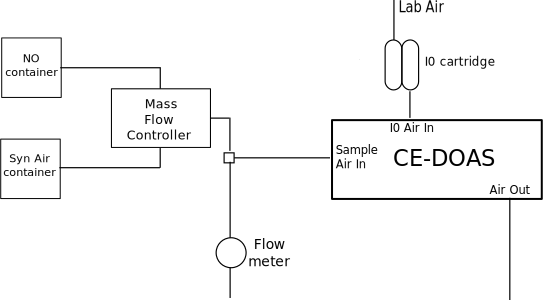
\includegraphics[width=0.6\textwidth]{no_setup.png}
  \caption{Setup of the calibration measurement}
  \label{fig:no-setup}
\end{figure}

To later be able to compare the measured \ch{NO} concentration we have
to convert the applied \ch{NO} flow to a concentration, too. We can
do this using the following formula
\begin{align*}
  c_{\ch{NO}} = c_{\text{cont}} \cdot \frac{\Phi_{\ch{NO}}}{\Phi_{\text{air}} + \Phi_{\ch{NO}}}
\end{align*}

with the concentration $c_{\text{cont}}$ in the \ch{NO} container
given to be \SI{8.177}{ppb}. 

\subsection{Measurement results}
\label{sec:no-result}

Figure~\ref{fig:ts} Shows the timeseries of the \ch{NO} and \ch{O3}
concentration. Each of the three clusters corresponds from left to
right to the reaction path length of \num{5}, \num{10} and
\SI{15}{\meter}. The Ozone concentration is within the margin of its
error constant while we see that the overall shape of the \ch{NO}
timeseries does not depend on the pathlength. One deviation can be
found in the $l = \SI{5}{\meter}$ plot, where all the upward flanks
have a very long decay time before they reach the stable plateau.

\begin{figure}[htbp]
  \centering
  \includegraphics[width=0.45\textwidth]{20160222_NO_fixI0_NO_ts.png}
  \hfill
  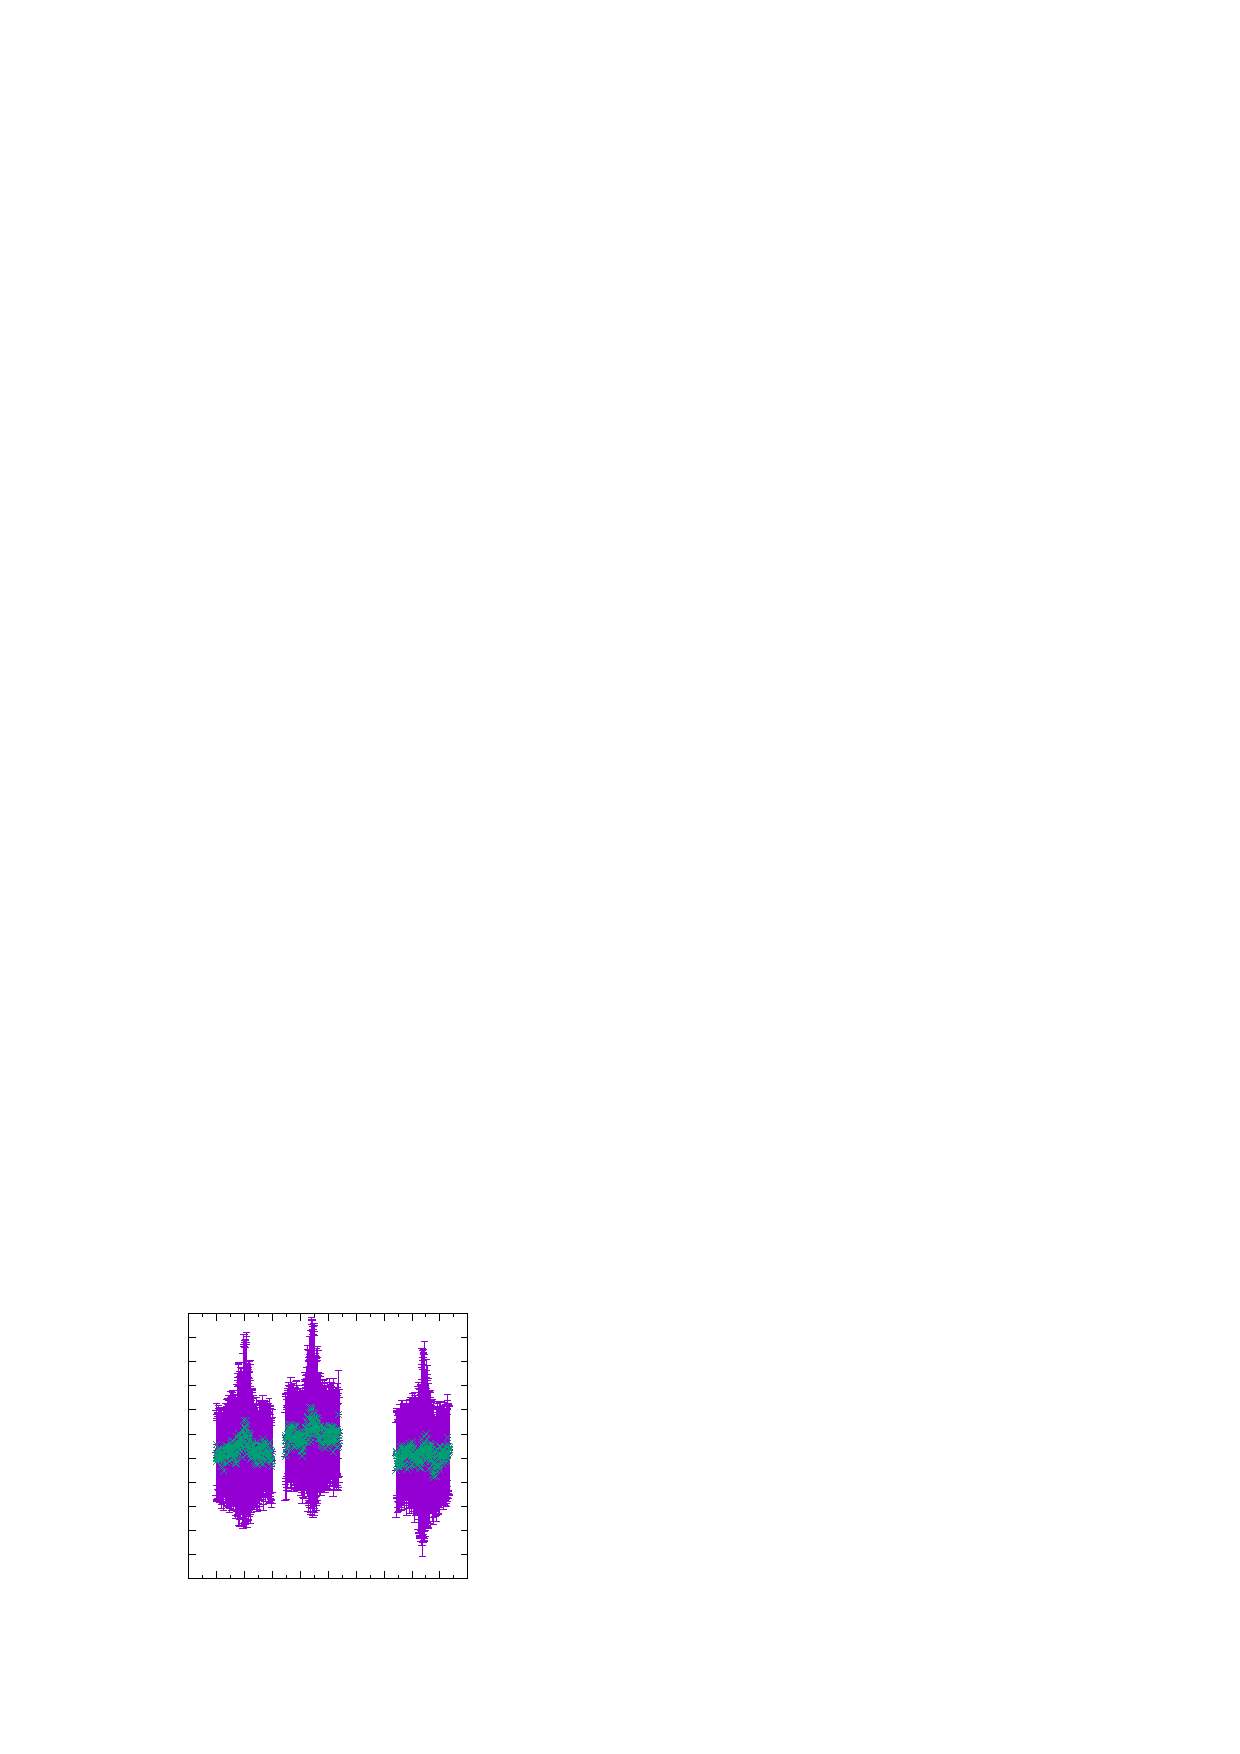
\includegraphics[width=0.45\textwidth]{20160222_NO_fixI0_O3_ts.png}
  \caption{Timeseries of the \ch{NO} and \ch{O3} concentration. The
    three clusters correspond to the three used reaction path lengths
    $l = 5, 10$ and \SI{15}{\meter}.}
  \label{fig:ts}
\end{figure}
\todo{Redo figures with sensible dimensions}

Averaging over regions of constant flow and plotting over the reaction
path length, we yield Figure~\ref{fig:no-length}. The figure also
contains linear interpolation of the data points. The plots together
with the fits imply that the measured \ch{NO} concentration does not
depend on the pathlength, as is well expected.

\begin{figure}[htbp]
  \centering
  \includegraphics[width=0.75\textwidth]{20160222_NO_fixI0_NO_length.png}
  \caption{\ch{NO} concentration dependence on reaction path
    length. The data points are colored depending on the applied
    \ch{NO} flow. All data points were linearly interpolated. The
    results can also be found in the plot.}
  \label{fig:no-length}
\end{figure}

Since all measured concentration are pathlength independent, we can
all use them to compare the measured \ch{NO} concentration to the
computed \ch{NO} concentration. The summary is shown in
Figure~\ref{fig:no-calib}. The linear regression line follows the formula

\begin{align*}
  y = 0.994 \cdot x -0.00234.
\end{align*}

This is an exceptional accordance between the measured and the
computed mixing ratios.

\begin{figure}[htbp]
  \centering
  \includegraphics[width=0.75\textwidth]{20160222_NO_fixI0.png}
  \caption{Correlation plot of the computed and the measured \ch{pNO}
    concentration.}
  \label{fig:no-calib}
\end{figure}

%%% Local Variables:
%%% mode: latex
%%% TeX-master: "../Bachelor"
%%% End:

\cleardoubleoddstandardpage{}
\subsection{Comparison to chemiluminescence measurements}
\label{sec:cld}

After having assured the functionality of the converter in the lab
environment, I wanted to use it with ambient air. I wanted to try out
the alternating measurement mode described in the previous section and
compare the results to another nitrogen monoxide measurement
instrument, a chemiluminescence monitor (or display, short: cld). This
made it possible to work in a more realistic setting while
simultaneously being able to verify the converter results.

\subsubsection{Setup}
\label{sec:cld-setup}

The cavity and the chemiluminescence monitor (Eco Physics CLD 770 AL
ppt Chemiluminescence \ch{NO} Analyzer) were both setup at the rooftop
laboratory at the Institute for Environmental Physics. I used a
tripod on the roof together with two teflon tubes to make sure to
sample at the same spot with both instruments.

I set up the cavity as described in Section~\ref{sec:inclusion}. For
each spectrum I sampled 3000 spectra at an exposure time of
\SI{10}{\milli\second}. Furthermore, I used a purge time of
\SI{30}{\second} after ozone switches. This time was set too short to
account for the slowly falling tail, as Section~\ref{sec:switch}
indicates.

In order to account for slight differences in the path length and
flows in the two instruments, I decided to compute \SI{30}{\minute}
averages for the comparison. These measurements were taken during the
day of January 22 and January 25, 2016.

\subsubsection{Results}
\label{sec:cld-results}

The time series of the two measurements can be found in
Figure~\ref{fig:corr-ts}. As can be seen, the qualitative form of the
DOAS results is in good accordance with the chemiluminescence results.
However, there seems to be an offset and the DOAS concentration is
systematically lower than the chemiluminescence concentration. This
relation is also plainly visible in the correlation plot in
Figure~\ref{fig:cld-corr}. The measurements are very well correlated
and can be easily fitted by a linear regression, but the line has an
offset and a slope, which is differing from unity:

\begin{align*}
  y = \SI{1.38}{{ppb}\tothe{-1}} \cdot x + 3.8.
\end{align*}

There were two avenues I followed in an attempt to understand these
findings. Both of them follow arguments already layed out in
Section~\ref{sec:switch}. The first consists in the observation, that
the \ch{NO} calibration gas container was used to calibrate the
chemiluminescence display. If some of the \ch{NO} had been converted
to \ch{NO2}, there would be an error in the chemiluminescence
calibration, which would lead an overestimation of the \ch{NO}
concentration by the cld. Using the \ch{NO2}
offset found in the previous section, one can compute that there is
about \SI{420}{ppb} \ch{NO2} in the cylinder, if all of it stemmed
from \ch{NO} this would introduce an error of about \SI{5}{\percent}
(the calibration concentration given was $c = \SI{8.177}{ppm}$). This
is not enough to explain the discrepancy. Together with the fact that
I could not explain, how the transition from \ch{NO} to \ch{NO2} could
occur, I discarded this approach.

The second avenue I took, was to look at the purge time.
Section~\ref{sec:switch} suggests that \SI{30}{\second} purge time is
not enough after the ozone switch has been turned off. Thus one would
expect the measured \ch{NO2} intensities to be overestimated. One
observation pointing towards the influence of this effect ist, that I
measured negative \ch{NO} concentrations (to a minimum of
\SI{-1.54}{ppb}), which is of course absurd. In the previous section I
suggest, that the surplus \ch{NO2} signal does not depend too strongly
on the \ch{NO} concentration. If this assumption is correct, one will
expect to be able to mitigate the effects by lowering the \ch{NO2}
signal by $\bar c_s = \SI{1.55}{ppb}$ (c.\,f.\
Equation~\eqref{eq:offset} on page~\pageref{eq:offset}), which
corresponds surprisingly well to the negative offset of the measured
data. This \emph{tail corrected} data set was then again correlated
with the chemiluminescence data. The result can also be found in
Figure~\ref{fig:cld-corr}. The linear regression follows the formula
\begin{align*}
  y = \SI{1.38}{ppb\tothe{-1}} \cdot x + 1.67.
\end{align*}
So the tail correction has only an effect on the
intercept of the regression. This is expected as the constant lowering
of the \ch{NO2} signal increases the computed \ch{NO} signal by the
same amount and thus all data points are shifted to the
right. Hence the slope of the regression is still off. Clearly the
aprroach utilized here was too simplistic to account for all
effects. Further investigations are necessary to understand the
corrections necessary. Possibly, the \ch{NO2} correction can be
computed utilizing the previous \ch{NO_x} data point, thus indirectly
taking \ch{NO} influences on the offset into account. This varying \ch{NO2}
correction could then also influence the slope of the
regression. In order to investigate this further I suggest to perform
additional decay measurements as proposed in the previous section.

\begin{figure}[htbp]
  \centering
  % GNUPLOT: LaTeX picture with Postscript
\begingroup
  \makeatletter
  \providecommand\color[2][]{%
    \GenericError{(gnuplot) \space\space\space\@spaces}{%
      Package color not loaded in conjunction with
      terminal option `colourtext'%
    }{See the gnuplot documentation for explanation.%
    }{Either use 'blacktext' in gnuplot or load the package
      color.sty in LaTeX.}%
    \renewcommand\color[2][]{}%
  }%
  \providecommand\includegraphics[2][]{%
    \GenericError{(gnuplot) \space\space\space\@spaces}{%
      Package graphicx or graphics not loaded%
    }{See the gnuplot documentation for explanation.%
    }{The gnuplot epslatex terminal needs graphicx.sty or graphics.sty.}%
    \renewcommand\includegraphics[2][]{}%
  }%
  \providecommand\rotatebox[2]{#2}%
  \@ifundefined{ifGPcolor}{%
    \newif\ifGPcolor
    \GPcolorfalse
  }{}%
  \@ifundefined{ifGPblacktext}{%
    \newif\ifGPblacktext
    \GPblacktexttrue
  }{}%
  % define a \g@addto@macro without @ in the name:
  \let\gplgaddtomacro\g@addto@macro
  % define empty templates for all commands taking text:
  \gdef\gplbacktext{}%
  \gdef\gplfronttext{}%
  \makeatother
  \ifGPblacktext
    % no textcolor at all
    \def\colorrgb#1{}%
    \def\colorgray#1{}%
  \else
    % gray or color?
    \ifGPcolor
      \def\colorrgb#1{\color[rgb]{#1}}%
      \def\colorgray#1{\color[gray]{#1}}%
      \expandafter\def\csname LTw\endcsname{\color{white}}%
      \expandafter\def\csname LTb\endcsname{\color{black}}%
      \expandafter\def\csname LTa\endcsname{\color{black}}%
      \expandafter\def\csname LT0\endcsname{\color[rgb]{1,0,0}}%
      \expandafter\def\csname LT1\endcsname{\color[rgb]{0,1,0}}%
      \expandafter\def\csname LT2\endcsname{\color[rgb]{0,0,1}}%
      \expandafter\def\csname LT3\endcsname{\color[rgb]{1,0,1}}%
      \expandafter\def\csname LT4\endcsname{\color[rgb]{0,1,1}}%
      \expandafter\def\csname LT5\endcsname{\color[rgb]{1,1,0}}%
      \expandafter\def\csname LT6\endcsname{\color[rgb]{0,0,0}}%
      \expandafter\def\csname LT7\endcsname{\color[rgb]{1,0.3,0}}%
      \expandafter\def\csname LT8\endcsname{\color[rgb]{0.5,0.5,0.5}}%
    \else
      % gray
      \def\colorrgb#1{\color{black}}%
      \def\colorgray#1{\color[gray]{#1}}%
      \expandafter\def\csname LTw\endcsname{\color{white}}%
      \expandafter\def\csname LTb\endcsname{\color{black}}%
      \expandafter\def\csname LTa\endcsname{\color{black}}%
      \expandafter\def\csname LT0\endcsname{\color{black}}%
      \expandafter\def\csname LT1\endcsname{\color{black}}%
      \expandafter\def\csname LT2\endcsname{\color{black}}%
      \expandafter\def\csname LT3\endcsname{\color{black}}%
      \expandafter\def\csname LT4\endcsname{\color{black}}%
      \expandafter\def\csname LT5\endcsname{\color{black}}%
      \expandafter\def\csname LT6\endcsname{\color{black}}%
      \expandafter\def\csname LT7\endcsname{\color{black}}%
      \expandafter\def\csname LT8\endcsname{\color{black}}%
    \fi
  \fi
    \setlength{\unitlength}{0.0500bp}%
    \ifx\gptboxheight\undefined%
      \newlength{\gptboxheight}%
      \newlength{\gptboxwidth}%
      \newsavebox{\gptboxtext}%
    \fi%
    \setlength{\fboxrule}{0.5pt}%
    \setlength{\fboxsep}{1pt}%
\begin{picture}(4030.00,4030.00)%
    \gplgaddtomacro\gplbacktext{%
      \csname LTb\endcsname%
      \put(682,686){\makebox(0,0)[r]{\strut{}$-5$}}%
      \put(682,954){\makebox(0,0)[r]{\strut{}$0$}}%
      \put(682,1223){\makebox(0,0)[r]{\strut{}$5$}}%
      \put(682,1491){\makebox(0,0)[r]{\strut{}$10$}}%
      \put(682,1759){\makebox(0,0)[r]{\strut{}$15$}}%
      \put(682,2028){\makebox(0,0)[r]{\strut{}$20$}}%
      \put(682,2296){\makebox(0,0)[r]{\strut{}$25$}}%
      \put(682,2564){\makebox(0,0)[r]{\strut{}$30$}}%
      \put(682,2832){\makebox(0,0)[r]{\strut{}$35$}}%
      \put(682,3101){\makebox(0,0)[r]{\strut{}$40$}}%
      \put(682,3369){\makebox(0,0)[r]{\strut{}$45$}}%
      \put(814,554){\rotatebox{-45}{\makebox(0,0)[l]{\strut{}16:00}}}%
      \put(1166,554){\rotatebox{-45}{\makebox(0,0)[l]{\strut{}17:00}}}%
      \put(1519,554){\rotatebox{-45}{\makebox(0,0)[l]{\strut{}18:00}}}%
      \put(1871,554){\rotatebox{-45}{\makebox(0,0)[l]{\strut{}19:00}}}%
      \put(2224,554){\rotatebox{-45}{\makebox(0,0)[l]{\strut{}20:00}}}%
      \put(2576,554){\rotatebox{-45}{\makebox(0,0)[l]{\strut{}21:00}}}%
      \put(2928,554){\rotatebox{-45}{\makebox(0,0)[l]{\strut{}22:00}}}%
      \put(3281,554){\rotatebox{-45}{\makebox(0,0)[l]{\strut{}23:00}}}%
      \put(3633,554){\rotatebox{-45}{\makebox(0,0)[l]{\strut{}00:00}}}%
    }%
    \gplgaddtomacro\gplfronttext{%
      \csname LTb\endcsname%
      \put(176,2027){\rotatebox{-270}{\makebox(0,0){\strut{}Concentration [ppb]}}}%
      \put(2223,3699){\makebox(0,0){\strut{}January 22, 2016}}%
      \csname LTb\endcsname%
      \put(1474,3196){\makebox(0,0)[r]{\strut{}DOAS}}%
      \csname LTb\endcsname%
      \put(1474,2976){\makebox(0,0)[r]{\strut{}CL}}%
    }%
    \gplbacktext
    \put(0,0){\includegraphics{../images/correlation_ts01}}%
    \gplfronttext
  \end{picture}%
\endgroup

  \hfill
  % GNUPLOT: LaTeX picture with Postscript
\begingroup
  \makeatletter
  \providecommand\color[2][]{%
    \GenericError{(gnuplot) \space\space\space\@spaces}{%
      Package color not loaded in conjunction with
      terminal option `colourtext'%
    }{See the gnuplot documentation for explanation.%
    }{Either use 'blacktext' in gnuplot or load the package
      color.sty in LaTeX.}%
    \renewcommand\color[2][]{}%
  }%
  \providecommand\includegraphics[2][]{%
    \GenericError{(gnuplot) \space\space\space\@spaces}{%
      Package graphicx or graphics not loaded%
    }{See the gnuplot documentation for explanation.%
    }{The gnuplot epslatex terminal needs graphicx.sty or graphics.sty.}%
    \renewcommand\includegraphics[2][]{}%
  }%
  \providecommand\rotatebox[2]{#2}%
  \@ifundefined{ifGPcolor}{%
    \newif\ifGPcolor
    \GPcolorfalse
  }{}%
  \@ifundefined{ifGPblacktext}{%
    \newif\ifGPblacktext
    \GPblacktexttrue
  }{}%
  % define a \g@addto@macro without @ in the name:
  \let\gplgaddtomacro\g@addto@macro
  % define empty templates for all commands taking text:
  \gdef\gplbacktext{}%
  \gdef\gplfronttext{}%
  \makeatother
  \ifGPblacktext
    % no textcolor at all
    \def\colorrgb#1{}%
    \def\colorgray#1{}%
  \else
    % gray or color?
    \ifGPcolor
      \def\colorrgb#1{\color[rgb]{#1}}%
      \def\colorgray#1{\color[gray]{#1}}%
      \expandafter\def\csname LTw\endcsname{\color{white}}%
      \expandafter\def\csname LTb\endcsname{\color{black}}%
      \expandafter\def\csname LTa\endcsname{\color{black}}%
      \expandafter\def\csname LT0\endcsname{\color[rgb]{1,0,0}}%
      \expandafter\def\csname LT1\endcsname{\color[rgb]{0,1,0}}%
      \expandafter\def\csname LT2\endcsname{\color[rgb]{0,0,1}}%
      \expandafter\def\csname LT3\endcsname{\color[rgb]{1,0,1}}%
      \expandafter\def\csname LT4\endcsname{\color[rgb]{0,1,1}}%
      \expandafter\def\csname LT5\endcsname{\color[rgb]{1,1,0}}%
      \expandafter\def\csname LT6\endcsname{\color[rgb]{0,0,0}}%
      \expandafter\def\csname LT7\endcsname{\color[rgb]{1,0.3,0}}%
      \expandafter\def\csname LT8\endcsname{\color[rgb]{0.5,0.5,0.5}}%
    \else
      % gray
      \def\colorrgb#1{\color{black}}%
      \def\colorgray#1{\color[gray]{#1}}%
      \expandafter\def\csname LTw\endcsname{\color{white}}%
      \expandafter\def\csname LTb\endcsname{\color{black}}%
      \expandafter\def\csname LTa\endcsname{\color{black}}%
      \expandafter\def\csname LT0\endcsname{\color{black}}%
      \expandafter\def\csname LT1\endcsname{\color{black}}%
      \expandafter\def\csname LT2\endcsname{\color{black}}%
      \expandafter\def\csname LT3\endcsname{\color{black}}%
      \expandafter\def\csname LT4\endcsname{\color{black}}%
      \expandafter\def\csname LT5\endcsname{\color{black}}%
      \expandafter\def\csname LT6\endcsname{\color{black}}%
      \expandafter\def\csname LT7\endcsname{\color{black}}%
      \expandafter\def\csname LT8\endcsname{\color{black}}%
    \fi
  \fi
    \setlength{\unitlength}{0.0500bp}%
    \ifx\gptboxheight\undefined%
      \newlength{\gptboxheight}%
      \newlength{\gptboxwidth}%
      \newsavebox{\gptboxtext}%
    \fi%
    \setlength{\fboxrule}{0.5pt}%
    \setlength{\fboxsep}{1pt}%
\begin{picture}(3888.00,3888.00)%
    \gplgaddtomacro\gplbacktext{%
      \csname LTb\endcsname%
      \put(814,686){\makebox(0,0)[r]{\strut{}$-10$}}%
      \put(814,1049){\makebox(0,0)[r]{\strut{}$0$}}%
      \put(814,1412){\makebox(0,0)[r]{\strut{}$10$}}%
      \put(814,1775){\makebox(0,0)[r]{\strut{}$20$}}%
      \put(814,2138){\makebox(0,0)[r]{\strut{}$30$}}%
      \put(814,2501){\makebox(0,0)[r]{\strut{}$40$}}%
      \put(814,2864){\makebox(0,0)[r]{\strut{}$50$}}%
      \put(814,3227){\makebox(0,0)[r]{\strut{}$60$}}%
      \put(946,554){\rotatebox{-45}{\makebox(0,0)[l]{\strut{}08:00}}}%
      \put(1264,554){\rotatebox{-45}{\makebox(0,0)[l]{\strut{}10:00}}}%
      \put(1582,554){\rotatebox{-45}{\makebox(0,0)[l]{\strut{}12:00}}}%
      \put(1900,554){\rotatebox{-45}{\makebox(0,0)[l]{\strut{}14:00}}}%
      \put(2219,554){\rotatebox{-45}{\makebox(0,0)[l]{\strut{}16:00}}}%
      \put(2537,554){\rotatebox{-45}{\makebox(0,0)[l]{\strut{}18:00}}}%
      \put(2855,554){\rotatebox{-45}{\makebox(0,0)[l]{\strut{}20:00}}}%
      \put(3173,554){\rotatebox{-45}{\makebox(0,0)[l]{\strut{}22:00}}}%
      \put(3491,554){\rotatebox{-45}{\makebox(0,0)[l]{\strut{}00:00}}}%
    }%
    \gplgaddtomacro\gplfronttext{%
      \csname LTb\endcsname%
      \put(176,1956){\rotatebox{-270}{\makebox(0,0){\strut{}\ch{NO} Concentration [ppb]}}}%
      \put(2218,3557){\makebox(0,0){\strut{}January 25, 2016}}%
      \csname LTb\endcsname%
      \put(2504,3054){\makebox(0,0)[r]{\strut{}ICAD}}%
      \csname LTb\endcsname%
      \put(2504,2834){\makebox(0,0)[r]{\strut{}CLD}}%
    }%
    \gplbacktext
    \put(0,0){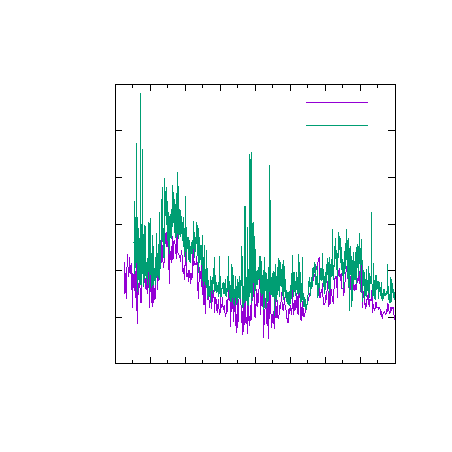
\includegraphics{../images/correlation_ts02}}%
    \gplfronttext
  \end{picture}%
\endgroup

  \caption{Time series of the \ch{NO} concentration during the two
    measurements on January 22 and January 25. Green depicts the
    chemiluminescence measurement, violet the DOAS measurement.}
  \label{fig:corr-ts}
\end{figure}
\begin{figure}[htbp]
  \centering
  \input{images/Correlation_corrected}
  \caption{Correlation plot between the DOAS instrument and a
    chemiluminescence monitor (CLD). Each data point depicts a
    \SI{30}{\minute} average.}
  \label{fig:cld-corr}
\end{figure}

All in all it seems that there are a few more stumbling blocks ahead
before this alternating measurement mode is ready for productive
use. The behaviour of the converter after an ozone switch has to be
characterized thoroughly to explain and cope with all the observed
effects.

%%% Local Variables:
%%% mode: latex
%%% TeX-master: "../Bachelor"
%%% End:

\cleardoubleoddstandardpage{}
\subsection{Vehicle measurements}
\label{sec:vehicle}

During this last measurement, I wanted to test the converter under the
conditions of in vivo vehicle measurements. The great advantage of
such measurements is that the European guidelines for nitrogen oxide
emission (the so called Euro 6 norms) are only concerned with
\ch{NO_x} (c.\,f.~\cite{eu}), i.\,e.\ in this case it is not necessary
to separate \ch{NO} from \ch{NO2}. Still, I wanted to compare the
\ch{NO_x} results to the results of pure \ch{NO2} measurements to
gauge the influence of the additional \ch{NO} on the air
pollution. Therefore, two cavities were used in parallel. One with the
converter, the other one without. With this very comfortable setup I
could even compute the \ch{NO} concentration without having to turn
the ozone on and off, which mitigated all the undesired effects
described in the previous two sections.

\subsubsection{Setup}
\label{sec:vehicle-setup}

For the measurement a car was loaded with both ICAD instruments and
the pickup tube was attached directly above the front license
plate. The main ideas behind the setup can be found in
Figure~\ref{fig:hd-principle}, where the institute's bus was equipped
with an ICAD instrument. The \ch{NO_x} cell was set up according to
Section~\ref{sec:inclusion} with an exposure time of
\SI{10}{\milli\second} and 100 scans per spectrum leading to a time
resolution of \SI{1}{\second}. As \ch{NO2} instrument I used the
AQM$_{\text{Tec}}$ Compact ICAD, which is the standard instrument at
the Institute for Environmental Physics for \ch{NO2} measurements in
urban areas and especially vehicle measurements. This \ch{NO2} ICAD
operated at a \SI{2}{\second} time resolution and had the further
advantage of possessing a \ch{CO2} sensor. This allowed the
computation of the ratios between nitrogen (di-)oxide and carbon
dioxide, which are a good measure for the emission per (gazoline)
consumption of the vehicles.

\begin{figure}[htbp]
  \centering
  \includegraphics[width=0.8\textwidth]{vehicle_principle.jpg}
  \caption{Principle setup behind the vehicle measurements. Instead of
    the institute's bus a car was equipped with the ICAD
    instruments. The picture was provided by~\cite{denis}.}
  \label{fig:hd-principle}
\end{figure}

The measurements took place on Friday, February 05, 2016 in Heidelberg
between 11:00 and 16:30. From 12:15 to 13:45, I operated both
measurement cells in \ch{NO2} mode to test for systematic
deviations. From 15:00 to 16:00, the measurement vehicle was
positioned next to the Heidelberg air quality measurement station to
be able to compare the \ch{NO} and \ch{NO2} values to the ones of the
station as a test of reliability. In between, 30 vehicles were
observed throughout Heidelberg for {\nfrac{} 1/2}~\si{\minute} to
\SI{10}{\minute} each.  Since the two cavities' clocks could not be
fully synchronized, the time series had to be matched in the
evaluation process. This was done manually using succinct peaks in the
plots.

\begin{figure}[htbp]
  \centering
  % GNUPLOT: LaTeX picture with Postscript
\begingroup
  \makeatletter
  \providecommand\color[2][]{%
    \GenericError{(gnuplot) \space\space\space\@spaces}{%
      Package color not loaded in conjunction with
      terminal option `colourtext'%
    }{See the gnuplot documentation for explanation.%
    }{Either use 'blacktext' in gnuplot or load the package
      color.sty in LaTeX.}%
    \renewcommand\color[2][]{}%
  }%
  \providecommand\includegraphics[2][]{%
    \GenericError{(gnuplot) \space\space\space\@spaces}{%
      Package graphicx or graphics not loaded%
    }{See the gnuplot documentation for explanation.%
    }{The gnuplot epslatex terminal needs graphicx.sty or graphics.sty.}%
    \renewcommand\includegraphics[2][]{}%
  }%
  \providecommand\rotatebox[2]{#2}%
  \@ifundefined{ifGPcolor}{%
    \newif\ifGPcolor
    \GPcolorfalse
  }{}%
  \@ifundefined{ifGPblacktext}{%
    \newif\ifGPblacktext
    \GPblacktexttrue
  }{}%
  % define a \g@addto@macro without @ in the name:
  \let\gplgaddtomacro\g@addto@macro
  % define empty templates for all commands taking text:
  \gdef\gplbacktext{}%
  \gdef\gplfronttext{}%
  \makeatother
  \ifGPblacktext
    % no textcolor at all
    \def\colorrgb#1{}%
    \def\colorgray#1{}%
  \else
    % gray or color?
    \ifGPcolor
      \def\colorrgb#1{\color[rgb]{#1}}%
      \def\colorgray#1{\color[gray]{#1}}%
      \expandafter\def\csname LTw\endcsname{\color{white}}%
      \expandafter\def\csname LTb\endcsname{\color{black}}%
      \expandafter\def\csname LTa\endcsname{\color{black}}%
      \expandafter\def\csname LT0\endcsname{\color[rgb]{1,0,0}}%
      \expandafter\def\csname LT1\endcsname{\color[rgb]{0,1,0}}%
      \expandafter\def\csname LT2\endcsname{\color[rgb]{0,0,1}}%
      \expandafter\def\csname LT3\endcsname{\color[rgb]{1,0,1}}%
      \expandafter\def\csname LT4\endcsname{\color[rgb]{0,1,1}}%
      \expandafter\def\csname LT5\endcsname{\color[rgb]{1,1,0}}%
      \expandafter\def\csname LT6\endcsname{\color[rgb]{0,0,0}}%
      \expandafter\def\csname LT7\endcsname{\color[rgb]{1,0.3,0}}%
      \expandafter\def\csname LT8\endcsname{\color[rgb]{0.5,0.5,0.5}}%
    \else
      % gray
      \def\colorrgb#1{\color{black}}%
      \def\colorgray#1{\color[gray]{#1}}%
      \expandafter\def\csname LTw\endcsname{\color{white}}%
      \expandafter\def\csname LTb\endcsname{\color{black}}%
      \expandafter\def\csname LTa\endcsname{\color{black}}%
      \expandafter\def\csname LT0\endcsname{\color{black}}%
      \expandafter\def\csname LT1\endcsname{\color{black}}%
      \expandafter\def\csname LT2\endcsname{\color{black}}%
      \expandafter\def\csname LT3\endcsname{\color{black}}%
      \expandafter\def\csname LT4\endcsname{\color{black}}%
      \expandafter\def\csname LT5\endcsname{\color{black}}%
      \expandafter\def\csname LT6\endcsname{\color{black}}%
      \expandafter\def\csname LT7\endcsname{\color{black}}%
      \expandafter\def\csname LT8\endcsname{\color{black}}%
    \fi
  \fi
    \setlength{\unitlength}{0.0500bp}%
    \ifx\gptboxheight\undefined%
      \newlength{\gptboxheight}%
      \newlength{\gptboxwidth}%
      \newsavebox{\gptboxtext}%
    \fi%
    \setlength{\fboxrule}{0.5pt}%
    \setlength{\fboxsep}{1pt}%
\begin{picture}(7776.00,4320.00)%
    \gplgaddtomacro\gplbacktext{%
      \csname LTb\endcsname%
      \put(682,440){\makebox(0,0)[r]{\strut{}$10$}}%
      \put(682,892){\makebox(0,0)[r]{\strut{}$20$}}%
      \put(682,1344){\makebox(0,0)[r]{\strut{}$30$}}%
      \put(682,1796){\makebox(0,0)[r]{\strut{}$40$}}%
      \put(682,2248){\makebox(0,0)[r]{\strut{}$50$}}%
      \put(682,2699){\makebox(0,0)[r]{\strut{}$60$}}%
      \put(682,3151){\makebox(0,0)[r]{\strut{}$70$}}%
      \put(682,3603){\makebox(0,0)[r]{\strut{}$80$}}%
      \put(682,4055){\makebox(0,0)[r]{\strut{}$90$}}%
      \put(814,220){\makebox(0,0){\strut{}12:10}}%
      \put(1471,220){\makebox(0,0){\strut{}12:20}}%
      \put(2127,220){\makebox(0,0){\strut{}12:30}}%
      \put(2784,220){\makebox(0,0){\strut{}12:40}}%
      \put(3440,220){\makebox(0,0){\strut{}12:50}}%
      \put(4097,220){\makebox(0,0){\strut{}13:00}}%
      \put(4753,220){\makebox(0,0){\strut{}13:10}}%
      \put(5410,220){\makebox(0,0){\strut{}13:20}}%
      \put(6066,220){\makebox(0,0){\strut{}13:30}}%
      \put(6723,220){\makebox(0,0){\strut{}13:40}}%
      \put(7379,220){\makebox(0,0){\strut{}13:50}}%
    }%
    \gplgaddtomacro\gplfronttext{%
      \csname LTb\endcsname%
      \put(176,2247){\rotatebox{-270}{\makebox(0,0){\strut{}\ch{NO2} Concentration [ppb]}}}%
      \csname LTb\endcsname%
      \put(6392,3882){\makebox(0,0)[r]{\strut{}\ch{NO2} ICAD }}%
      \csname LTb\endcsname%
      \put(6392,3662){\makebox(0,0)[r]{\strut{}\ch{NO_x} ICAD}}%
    }%
    \gplbacktext
    \put(0,0){\includegraphics{../images/hd_comparison}}%
    \gplfronttext
  \end{picture}%
\endgroup

  \caption{Comparison of the two used ICAD systems. Both were
    operated in pure \ch{NO2} measurement mode.}
  \label{fig:hd-comparison}
\end{figure}
\begin{figure}[htbp]
  \centering
  \input{images/vehicle_corr}
  \caption{Correlation between the two used ICAD systems. Both were
    operated in pur \ch{NO2} measurement mode. The data points depict
    \SI{1}{\minute} averages.}
  \label{fig:hd-corr}
\end{figure}

\subsubsection{Results}
\label{sec:vehicle-results}

In Figure~\ref{fig:hd-comparison} one can see that the measured
\ch{NO2} concentrations of the two cavities, which were then both
operated in \ch{NO2} mode. There seems to be no qualitative difference
between the two. However, the \ch{NO_x} cavity measured slightly lower
concentrations than the \ch{NO2} cavity. For a more precise analysis
the correlation between the two time series was
determined. Figure~\ref{fig:hd-corr} contains \SI{1}{\minute} averages
together with a linear regression, which follows the formula
\begin{align*}
  y = \num{0.99 \pm 0.01} \cdot x + \num{0.6 \pm 0.3}.
\end{align*}
Except for some data points on the left tail, the two time series seem
to be well correlated. The slope of the regression coincides with
unity within its uncertainty, but the intercept differs from
zero. Regarding the consequences of this finding, this offset is not
large absolutely speaking, but the question remains why it exists at
all. The most probable explanation is that the zero air spectrum used
in the evaluation of the \ch{NO_x} cavity was not completely trace gas
free. One reason that points towards this direction is that in the
\ch{NO_x} measurement mode there is a constant flow through the zero
air input, as this is the input for the ozone generator, too. Thus the
zero air filter is much more strained than it would be in a cavity
without \ch{NO_x} mode. Since the cavity had been thoroughly tested
for multiple weeks, starting effects of a saturation of the silica gel
or the activated carbon seem plausible.

For the comparison to the air quality measurement station, this effect
might be of interest as the deviation is large enough in this
case. During the vehicle measurements it should well be negligible as
the measured concentrations lay in the region of several hundered
\si{ppb} (see below). Additionally, the value is small compared to
other uncertainties affecting the concentrations there (e.\,g.\ the
influence of the varying distance to the measured vehicle or of the
neighbouring traffic).

\begin{figure}[htbp]
  \centering
  % GNUPLOT: LaTeX picture with Postscript
\begingroup
  \makeatletter
  \providecommand\color[2][]{%
    \GenericError{(gnuplot) \space\space\space\@spaces}{%
      Package color not loaded in conjunction with
      terminal option `colourtext'%
    }{See the gnuplot documentation for explanation.%
    }{Either use 'blacktext' in gnuplot or load the package
      color.sty in LaTeX.}%
    \renewcommand\color[2][]{}%
  }%
  \providecommand\includegraphics[2][]{%
    \GenericError{(gnuplot) \space\space\space\@spaces}{%
      Package graphicx or graphics not loaded%
    }{See the gnuplot documentation for explanation.%
    }{The gnuplot epslatex terminal needs graphicx.sty or graphics.sty.}%
    \renewcommand\includegraphics[2][]{}%
  }%
  \providecommand\rotatebox[2]{#2}%
  \@ifundefined{ifGPcolor}{%
    \newif\ifGPcolor
    \GPcolorfalse
  }{}%
  \@ifundefined{ifGPblacktext}{%
    \newif\ifGPblacktext
    \GPblacktexttrue
  }{}%
  % define a \g@addto@macro without @ in the name:
  \let\gplgaddtomacro\g@addto@macro
  % define empty templates for all commands taking text:
  \gdef\gplbacktext{}%
  \gdef\gplfronttext{}%
  \makeatother
  \ifGPblacktext
    % no textcolor at all
    \def\colorrgb#1{}%
    \def\colorgray#1{}%
  \else
    % gray or color?
    \ifGPcolor
      \def\colorrgb#1{\color[rgb]{#1}}%
      \def\colorgray#1{\color[gray]{#1}}%
      \expandafter\def\csname LTw\endcsname{\color{white}}%
      \expandafter\def\csname LTb\endcsname{\color{black}}%
      \expandafter\def\csname LTa\endcsname{\color{black}}%
      \expandafter\def\csname LT0\endcsname{\color[rgb]{1,0,0}}%
      \expandafter\def\csname LT1\endcsname{\color[rgb]{0,1,0}}%
      \expandafter\def\csname LT2\endcsname{\color[rgb]{0,0,1}}%
      \expandafter\def\csname LT3\endcsname{\color[rgb]{1,0,1}}%
      \expandafter\def\csname LT4\endcsname{\color[rgb]{0,1,1}}%
      \expandafter\def\csname LT5\endcsname{\color[rgb]{1,1,0}}%
      \expandafter\def\csname LT6\endcsname{\color[rgb]{0,0,0}}%
      \expandafter\def\csname LT7\endcsname{\color[rgb]{1,0.3,0}}%
      \expandafter\def\csname LT8\endcsname{\color[rgb]{0.5,0.5,0.5}}%
    \else
      % gray
      \def\colorrgb#1{\color{black}}%
      \def\colorgray#1{\color[gray]{#1}}%
      \expandafter\def\csname LTw\endcsname{\color{white}}%
      \expandafter\def\csname LTb\endcsname{\color{black}}%
      \expandafter\def\csname LTa\endcsname{\color{black}}%
      \expandafter\def\csname LT0\endcsname{\color{black}}%
      \expandafter\def\csname LT1\endcsname{\color{black}}%
      \expandafter\def\csname LT2\endcsname{\color{black}}%
      \expandafter\def\csname LT3\endcsname{\color{black}}%
      \expandafter\def\csname LT4\endcsname{\color{black}}%
      \expandafter\def\csname LT5\endcsname{\color{black}}%
      \expandafter\def\csname LT6\endcsname{\color{black}}%
      \expandafter\def\csname LT7\endcsname{\color{black}}%
      \expandafter\def\csname LT8\endcsname{\color{black}}%
    \fi
  \fi
    \setlength{\unitlength}{0.0500bp}%
    \ifx\gptboxheight\undefined%
      \newlength{\gptboxheight}%
      \newlength{\gptboxwidth}%
      \newsavebox{\gptboxtext}%
    \fi%
    \setlength{\fboxrule}{0.5pt}%
    \setlength{\fboxsep}{1pt}%
\begin{picture}(8062.00,4320.00)%
    \gplgaddtomacro\gplbacktext{%
      \csname LTb\endcsname%
      \put(814,440){\makebox(0,0)[r]{\strut{}$-10$}}%
      \put(814,842){\makebox(0,0)[r]{\strut{}$0$}}%
      \put(814,1243){\makebox(0,0)[r]{\strut{}$10$}}%
      \put(814,1645){\makebox(0,0)[r]{\strut{}$20$}}%
      \put(814,2047){\makebox(0,0)[r]{\strut{}$30$}}%
      \put(814,2448){\makebox(0,0)[r]{\strut{}$40$}}%
      \put(814,2850){\makebox(0,0)[r]{\strut{}$50$}}%
      \put(814,3252){\makebox(0,0)[r]{\strut{}$60$}}%
      \put(814,3653){\makebox(0,0)[r]{\strut{}$70$}}%
      \put(814,4055){\makebox(0,0)[r]{\strut{}$80$}}%
      \put(946,220){\makebox(0,0){\strut{}14:50}}%
      \put(1693,220){\makebox(0,0){\strut{}15:00}}%
      \put(2439,220){\makebox(0,0){\strut{}15:10}}%
      \put(3186,220){\makebox(0,0){\strut{}15:20}}%
      \put(3932,220){\makebox(0,0){\strut{}15:30}}%
      \put(4679,220){\makebox(0,0){\strut{}15:40}}%
      \put(5425,220){\makebox(0,0){\strut{}15:50}}%
      \put(6172,220){\makebox(0,0){\strut{}16:00}}%
      \put(6918,220){\makebox(0,0){\strut{}16:10}}%
      \put(7665,220){\makebox(0,0){\strut{}16:20}}%
    }%
    \gplgaddtomacro\gplfronttext{%
      \csname LTb\endcsname%
      \put(176,2247){\rotatebox{-270}{\makebox(0,0){\strut{}Concentration [ppb]}}}%
      \csname LTb\endcsname%
      \put(6678,3882){\makebox(0,0)[r]{\strut{}\ch{NO2}}}%
      \csname LTb\endcsname%
      \put(6678,3662){\makebox(0,0)[r]{\strut{}\ch{NO_x}}}%
      \csname LTb\endcsname%
      \put(6678,3442){\makebox(0,0)[r]{\strut{}\ch{NO_{\text{\hphantom{x}}}}}}%
    }%
    \gplbacktext
    \put(0,0){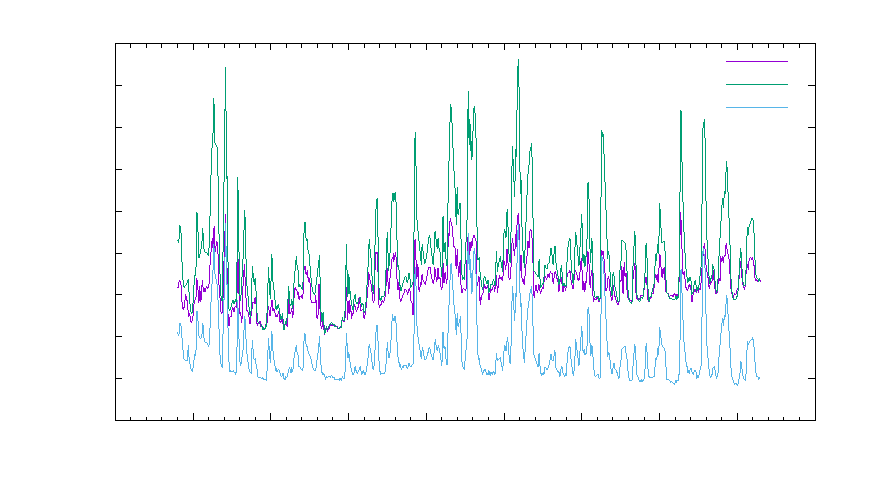
\includegraphics{../images/umba_ts}}%
    \gplfronttext
  \end{picture}%
\endgroup

  \caption{Timeseries of the \ch{NO_x}, \ch{NO2} and the computed
    \ch{NO} concentration next to the Umweltlandesamt air quality
    measurement station in Heidelberg.}
  \label{fig:umba}
\end{figure}

Figure~\ref{fig:umba} contains the time series of the measured
\ch{NO_x} and \ch{NO_2} and the computed \ch{NO} during the stay next
to the Heidelberg air quality measurement station. For moderate
\ch{NO2} concentrations between \num{10} and \SI{20}{ppb} the
\ch{NO_x} curve almost coincides with the \ch{NO2} curve. Only during
peaks there is a stronger separation and the \ch{NO_x} concentration
rises occasionally twice as high as the \ch{NO2} concentration. The
time series makes clear that neglecting \ch{NO} values while
estimating \ch{NO_x} pollution in urban areas can lead to serious
underestimation.

In a next step I computed the average concentrations for all three
time series and compared them to the station data taken
from~\cite{umba}. The results can be found in Table~\ref{tab:umba}. It
shows that there is a systematic deviation from the station, but the
values lie in the same region. The standard ICAD method has been
thoroughly tested during the last decades and is known to produce
solid results in good agreement with the measurement stations. Thus
the deviation of the \ch{NO2} average points towards outer influences
as explanations for the deviation. Indeed the pickup tube was about
\SI{3}{\meter} away from the station inlet and approximately
\SI{1}{\meter} lower (which means also closer to the driving
surface). These differences in the exact location can easily account
for the measured derivation.

Nevertheless, the main result remains that under field conditions in
ambient air the measured \ch{NO_x} and computed \ch{NO}
values are comparable to the ones of the station. This indicates once
more that the converter works and that if there is a second cavity at
hand, the setup seems to work very well for indirect \ch{NO}
measurements. Still, some more (and longer) measurements would be
advisable to acquire more data points for enough statistics to make a
comparison between the cavity and the station resilient.

\begin{table}[htbp]
  \centering
  \sisetup{
    table-format=2.1(2)
  }
  \begin{tabular}{l S S}
    \toprule
    {Compound} & \multicolumn{2}{c}{Concentration in \si{ppb}}\\
    & {Station} & {DOAS}\\
    \midrule
    \ch{NO} & 7.4 & 6.5 \pm 0.2\\
    \ch{NO2} & 19.2 & 21.9 \pm 0.1\\
    \ch{NOx} & 26.6 & 28.2 \pm 0.4\\ 
    \bottomrule
  \end{tabular}
  \caption{Comparison of the \SI{1}{\hour} \ch{NO}, \ch{NO2} and
    \ch{NO_x} averages from 15:00 to 16:00 on February 05, 2016
    between the air quality measurement station and the improved ICAD
    instrument. The station data was taken from~\cite{umba}; no
    uncertainties were provided.}
  \label{tab:umba}
\end{table}

In between the above described experiments, \num{30} vehicles were
measured within Heidelberg. The main result is that there is a large
discrepancy between the \ch{NO2} and \ch{NO_x} values. During peaks
the \ch{NO_x} values exceed the \ch{NO2} values by far.

As an in depth analysis of all vehicles would most likely go beyond
the scope of this thesis and furthermore miss the point of
characterizing and analyzing the converter, I will restrict my
attention to two exemplary vehicles. I chose these by reason of
pursuit time and distinguishability from background and ended up with
one diesel car and a public-transit bus. The first example is a
Mercedes B180 CDI.\@ The time series is depicted in
Figure~\ref{fig:mercedes-ts} and a picture of the vehicle together
with the surrounding traffic is shown in Figure~\ref{fig:bus}
left-hand side. There are five to six acceleration periods visible and
most prominent in the \ch{NO_x} time series. The \ch{NO_2} values vary
the least and are between a factor four and a factor nine smaller than
the \ch{NO_x} values during peaks. In the valleys between peaks, the
\ch{NO_x} approaches the \ch{NO2}, but is still significantly
higher. The \ch{CO2} time series has the same overall appearance as
the \ch{NO_x} curve. For a quantitave analysis the nitrogen (di-)oxide
emission per carbon dioxide emission is computed. Using the official
\ch{CO2} efficiency classes an emission of
\SI{150}{\gram\per\kilo\meter} of \ch{CO2} for the car is
obtained. Together with the molar masses of the species this can be
converted to the emission of \ch{NO2} and \ch{NO_x} respectively. The
results can be found in Table~\ref{tab:mercedes-bus}. It shows that
there is one order of magnitude difference between the corresponding
\ch{NO2} and \ch{NOx} values, which again underlines the blatant
underestimation of the vehicle emissions if only \ch{NO2} values are
taken into account.

\begin{figure}[htbp]
  \centering
  % GNUPLOT: LaTeX picture with Postscript
\begingroup
  \makeatletter
  \providecommand\color[2][]{%
    \GenericError{(gnuplot) \space\space\space\@spaces}{%
      Package color not loaded in conjunction with
      terminal option `colourtext'%
    }{See the gnuplot documentation for explanation.%
    }{Either use 'blacktext' in gnuplot or load the package
      color.sty in LaTeX.}%
    \renewcommand\color[2][]{}%
  }%
  \providecommand\includegraphics[2][]{%
    \GenericError{(gnuplot) \space\space\space\@spaces}{%
      Package graphicx or graphics not loaded%
    }{See the gnuplot documentation for explanation.%
    }{The gnuplot epslatex terminal needs graphicx.sty or graphics.sty.}%
    \renewcommand\includegraphics[2][]{}%
  }%
  \providecommand\rotatebox[2]{#2}%
  \@ifundefined{ifGPcolor}{%
    \newif\ifGPcolor
    \GPcolorfalse
  }{}%
  \@ifundefined{ifGPblacktext}{%
    \newif\ifGPblacktext
    \GPblacktexttrue
  }{}%
  % define a \g@addto@macro without @ in the name:
  \let\gplgaddtomacro\g@addto@macro
  % define empty templates for all commands taking text:
  \gdef\gplbacktext{}%
  \gdef\gplfronttext{}%
  \makeatother
  \ifGPblacktext
    % no textcolor at all
    \def\colorrgb#1{}%
    \def\colorgray#1{}%
  \else
    % gray or color?
    \ifGPcolor
      \def\colorrgb#1{\color[rgb]{#1}}%
      \def\colorgray#1{\color[gray]{#1}}%
      \expandafter\def\csname LTw\endcsname{\color{white}}%
      \expandafter\def\csname LTb\endcsname{\color{black}}%
      \expandafter\def\csname LTa\endcsname{\color{black}}%
      \expandafter\def\csname LT0\endcsname{\color[rgb]{1,0,0}}%
      \expandafter\def\csname LT1\endcsname{\color[rgb]{0,1,0}}%
      \expandafter\def\csname LT2\endcsname{\color[rgb]{0,0,1}}%
      \expandafter\def\csname LT3\endcsname{\color[rgb]{1,0,1}}%
      \expandafter\def\csname LT4\endcsname{\color[rgb]{0,1,1}}%
      \expandafter\def\csname LT5\endcsname{\color[rgb]{1,1,0}}%
      \expandafter\def\csname LT6\endcsname{\color[rgb]{0,0,0}}%
      \expandafter\def\csname LT7\endcsname{\color[rgb]{1,0.3,0}}%
      \expandafter\def\csname LT8\endcsname{\color[rgb]{0.5,0.5,0.5}}%
    \else
      % gray
      \def\colorrgb#1{\color{black}}%
      \def\colorgray#1{\color[gray]{#1}}%
      \expandafter\def\csname LTw\endcsname{\color{white}}%
      \expandafter\def\csname LTb\endcsname{\color{black}}%
      \expandafter\def\csname LTa\endcsname{\color{black}}%
      \expandafter\def\csname LT0\endcsname{\color{black}}%
      \expandafter\def\csname LT1\endcsname{\color{black}}%
      \expandafter\def\csname LT2\endcsname{\color{black}}%
      \expandafter\def\csname LT3\endcsname{\color{black}}%
      \expandafter\def\csname LT4\endcsname{\color{black}}%
      \expandafter\def\csname LT5\endcsname{\color{black}}%
      \expandafter\def\csname LT6\endcsname{\color{black}}%
      \expandafter\def\csname LT7\endcsname{\color{black}}%
      \expandafter\def\csname LT8\endcsname{\color{black}}%
    \fi
  \fi
    \setlength{\unitlength}{0.0500bp}%
    \ifx\gptboxheight\undefined%
      \newlength{\gptboxheight}%
      \newlength{\gptboxwidth}%
      \newsavebox{\gptboxtext}%
    \fi%
    \setlength{\fboxrule}{0.5pt}%
    \setlength{\fboxsep}{1pt}%
\begin{picture}(7200.00,5040.00)%
    \gplgaddtomacro\gplbacktext{%
      \csname LTb\endcsname%
      \put(946,966){\makebox(0,0)[r]{\strut{}$0$}}%
      \put(946,1347){\makebox(0,0)[r]{\strut{}$100$}}%
      \put(946,1728){\makebox(0,0)[r]{\strut{}$200$}}%
      \put(946,2109){\makebox(0,0)[r]{\strut{}$300$}}%
      \put(946,2490){\makebox(0,0)[r]{\strut{}$400$}}%
      \put(946,2871){\makebox(0,0)[r]{\strut{}$500$}}%
      \put(946,3251){\makebox(0,0)[r]{\strut{}$600$}}%
      \put(946,3632){\makebox(0,0)[r]{\strut{}$700$}}%
      \put(946,4013){\makebox(0,0)[r]{\strut{}$800$}}%
      \put(946,4394){\makebox(0,0)[r]{\strut{}$900$}}%
      \put(946,4775){\makebox(0,0)[r]{\strut{}$1000$}}%
      \put(1078,834){\rotatebox{-45}{\makebox(0,0)[l]{\strut{}11:15:00}}}%
      \put(1471,834){\rotatebox{-45}{\makebox(0,0)[l]{\strut{}11:15:30}}}%
      \put(1864,834){\rotatebox{-45}{\makebox(0,0)[l]{\strut{}11:16:00}}}%
      \put(2256,834){\rotatebox{-45}{\makebox(0,0)[l]{\strut{}11:16:30}}}%
      \put(2649,834){\rotatebox{-45}{\makebox(0,0)[l]{\strut{}11:17:00}}}%
      \put(3042,834){\rotatebox{-45}{\makebox(0,0)[l]{\strut{}11:17:30}}}%
      \put(3435,834){\rotatebox{-45}{\makebox(0,0)[l]{\strut{}11:18:00}}}%
      \put(3827,834){\rotatebox{-45}{\makebox(0,0)[l]{\strut{}11:18:30}}}%
      \put(4220,834){\rotatebox{-45}{\makebox(0,0)[l]{\strut{}11:19:00}}}%
      \put(4613,834){\rotatebox{-45}{\makebox(0,0)[l]{\strut{}11:19:30}}}%
      \put(5006,834){\rotatebox{-45}{\makebox(0,0)[l]{\strut{}11:20:00}}}%
      \put(5398,834){\rotatebox{-45}{\makebox(0,0)[l]{\strut{}11:20:30}}}%
      \put(5791,834){\rotatebox{-45}{\makebox(0,0)[l]{\strut{}11:21:00}}}%
      \put(5923,966){\makebox(0,0)[l]{\strut{}$0$}}%
      \put(5923,1347){\makebox(0,0)[l]{\strut{}$100$}}%
      \put(5923,1728){\makebox(0,0)[l]{\strut{}$200$}}%
      \put(5923,2109){\makebox(0,0)[l]{\strut{}$300$}}%
      \put(5923,2490){\makebox(0,0)[l]{\strut{}$400$}}%
      \put(5923,2871){\makebox(0,0)[l]{\strut{}$500$}}%
      \put(5923,3251){\makebox(0,0)[l]{\strut{}$600$}}%
      \put(5923,3632){\makebox(0,0)[l]{\strut{}$700$}}%
      \put(5923,4013){\makebox(0,0)[l]{\strut{}$800$}}%
      \put(5923,4394){\makebox(0,0)[l]{\strut{}$900$}}%
      \put(5923,4775){\makebox(0,0)[l]{\strut{}$1000$}}%
    }%
    \gplgaddtomacro\gplfronttext{%
      \csname LTb\endcsname%
      \put(176,2870){\rotatebox{-270}{\makebox(0,0){\strut{}\ch{NO2}/\ch{NO_x} Concentration [ppb]}}}%
      \put(6692,2870){\rotatebox{-270}{\makebox(0,0){\strut{}\ch{CO2} Concentration [ppm]}}}%
      \csname LTb\endcsname%
      \put(4804,4602){\makebox(0,0)[r]{\strut{}\ch{NO2}}}%
      \csname LTb\endcsname%
      \put(4804,4382){\makebox(0,0)[r]{\strut{}\ch{NO_x}}}%
      \csname LTb\endcsname%
      \put(4804,4162){\makebox(0,0)[r]{\strut{}\ch{CO2}}}%
    }%
    \gplbacktext
    \put(0,0){\includegraphics{../images/mercedes}}%
    \gplfronttext
  \end{picture}%
\endgroup

  \caption{Timeseries of the uncorrected \ch{NO2}, \ch{NO_x} and
    \ch{CO2} concentrations in the plume of a Mercedes B180 CDI.}
  \label{fig:mercedes-ts}
\end{figure}

\begin{figure}[htbp]
  \centering
  \includegraphics[width=0.45\textwidth]{mercedes.jpg}
  \hfill  
  \includegraphics[width=0.45\textwidth]{bus.jpg}
  \caption{Picture of the measured bus and Mercedes B180 CDI.\@{}Please note that
    the printed time is in utc.}
  \label{fig:bus}
\end{figure}

\begin{table}[hbtp]
  \sisetup{table-auto-round}
  \centering
  \begin{tabular}{lS[table-format=1.1(1)e-1]
    S[table-format=1.3(1)]
    S[table-format=1.1(1)e-1]
    S[table-format=1.2(1)]
    }
    \toprule
    & {\ch{NO2}/\ch{CO2}} & {\ch{NO2} emission} & {\ch{NO_x}/\ch{CO2}} &
                                                                   {\ch{NO_x}
                                                         emission}\\
    & & {\si{\gram\per\kilo\meter}} & & {\si{\gram\per\kilo\meter}}\\
    \midrule
    Mercedes & 2.2(3)e-4 & 0.034(5) & 5.0(7)e-3 & 0.53(7)\\
    Bus &  6(2)e-4 & 0.7(2) & 6(1)e-3 & 4.6(8)\\
    \bottomrule
  \end{tabular}
  \caption{\ch{NO2} and \ch{NO_x} to \ch{CO2} ratios together with the
    extrapolated emissions for the two vehicles.}
  \label{tab:mercedes-bus}
\end{table}

\begin{figure}[htbp]
  \centering
  % GNUPLOT: LaTeX picture with Postscript
\begingroup
  \makeatletter
  \providecommand\color[2][]{%
    \GenericError{(gnuplot) \space\space\space\@spaces}{%
      Package color not loaded in conjunction with
      terminal option `colourtext'%
    }{See the gnuplot documentation for explanation.%
    }{Either use 'blacktext' in gnuplot or load the package
      color.sty in LaTeX.}%
    \renewcommand\color[2][]{}%
  }%
  \providecommand\includegraphics[2][]{%
    \GenericError{(gnuplot) \space\space\space\@spaces}{%
      Package graphicx or graphics not loaded%
    }{See the gnuplot documentation for explanation.%
    }{The gnuplot epslatex terminal needs graphicx.sty or graphics.sty.}%
    \renewcommand\includegraphics[2][]{}%
  }%
  \providecommand\rotatebox[2]{#2}%
  \@ifundefined{ifGPcolor}{%
    \newif\ifGPcolor
    \GPcolorfalse
  }{}%
  \@ifundefined{ifGPblacktext}{%
    \newif\ifGPblacktext
    \GPblacktexttrue
  }{}%
  % define a \g@addto@macro without @ in the name:
  \let\gplgaddtomacro\g@addto@macro
  % define empty templates for all commands taking text:
  \gdef\gplbacktext{}%
  \gdef\gplfronttext{}%
  \makeatother
  \ifGPblacktext
    % no textcolor at all
    \def\colorrgb#1{}%
    \def\colorgray#1{}%
  \else
    % gray or color?
    \ifGPcolor
      \def\colorrgb#1{\color[rgb]{#1}}%
      \def\colorgray#1{\color[gray]{#1}}%
      \expandafter\def\csname LTw\endcsname{\color{white}}%
      \expandafter\def\csname LTb\endcsname{\color{black}}%
      \expandafter\def\csname LTa\endcsname{\color{black}}%
      \expandafter\def\csname LT0\endcsname{\color[rgb]{1,0,0}}%
      \expandafter\def\csname LT1\endcsname{\color[rgb]{0,1,0}}%
      \expandafter\def\csname LT2\endcsname{\color[rgb]{0,0,1}}%
      \expandafter\def\csname LT3\endcsname{\color[rgb]{1,0,1}}%
      \expandafter\def\csname LT4\endcsname{\color[rgb]{0,1,1}}%
      \expandafter\def\csname LT5\endcsname{\color[rgb]{1,1,0}}%
      \expandafter\def\csname LT6\endcsname{\color[rgb]{0,0,0}}%
      \expandafter\def\csname LT7\endcsname{\color[rgb]{1,0.3,0}}%
      \expandafter\def\csname LT8\endcsname{\color[rgb]{0.5,0.5,0.5}}%
    \else
      % gray
      \def\colorrgb#1{\color{black}}%
      \def\colorgray#1{\color[gray]{#1}}%
      \expandafter\def\csname LTw\endcsname{\color{white}}%
      \expandafter\def\csname LTb\endcsname{\color{black}}%
      \expandafter\def\csname LTa\endcsname{\color{black}}%
      \expandafter\def\csname LT0\endcsname{\color{black}}%
      \expandafter\def\csname LT1\endcsname{\color{black}}%
      \expandafter\def\csname LT2\endcsname{\color{black}}%
      \expandafter\def\csname LT3\endcsname{\color{black}}%
      \expandafter\def\csname LT4\endcsname{\color{black}}%
      \expandafter\def\csname LT5\endcsname{\color{black}}%
      \expandafter\def\csname LT6\endcsname{\color{black}}%
      \expandafter\def\csname LT7\endcsname{\color{black}}%
      \expandafter\def\csname LT8\endcsname{\color{black}}%
    \fi
  \fi
    \setlength{\unitlength}{0.0500bp}%
    \ifx\gptboxheight\undefined%
      \newlength{\gptboxheight}%
      \newlength{\gptboxwidth}%
      \newsavebox{\gptboxtext}%
    \fi%
    \setlength{\fboxrule}{0.5pt}%
    \setlength{\fboxsep}{1pt}%
\begin{picture}(7200.00,5040.00)%
    \gplgaddtomacro\gplbacktext{%
      \csname LTb\endcsname%
      \put(946,966){\makebox(0,0)[r]{\strut{}$0$}}%
      \put(946,1389){\makebox(0,0)[r]{\strut{}$500$}}%
      \put(946,1812){\makebox(0,0)[r]{\strut{}$1000$}}%
      \put(946,2236){\makebox(0,0)[r]{\strut{}$1500$}}%
      \put(946,2659){\makebox(0,0)[r]{\strut{}$2000$}}%
      \put(946,3082){\makebox(0,0)[r]{\strut{}$2500$}}%
      \put(946,3505){\makebox(0,0)[r]{\strut{}$3000$}}%
      \put(946,3929){\makebox(0,0)[r]{\strut{}$3500$}}%
      \put(946,4352){\makebox(0,0)[r]{\strut{}$4000$}}%
      \put(946,4775){\makebox(0,0)[r]{\strut{}$4500$}}%
      \put(1078,834){\rotatebox{-45}{\makebox(0,0)[l]{\strut{}14:25:00}}}%
      \put(1549,834){\rotatebox{-45}{\makebox(0,0)[l]{\strut{}14:26:00}}}%
      \put(2021,834){\rotatebox{-45}{\makebox(0,0)[l]{\strut{}14:27:00}}}%
      \put(2492,834){\rotatebox{-45}{\makebox(0,0)[l]{\strut{}14:28:00}}}%
      \put(2963,834){\rotatebox{-45}{\makebox(0,0)[l]{\strut{}14:29:00}}}%
      \put(3435,834){\rotatebox{-45}{\makebox(0,0)[l]{\strut{}14:30:00}}}%
      \put(3906,834){\rotatebox{-45}{\makebox(0,0)[l]{\strut{}14:31:00}}}%
      \put(4377,834){\rotatebox{-45}{\makebox(0,0)[l]{\strut{}14:32:00}}}%
      \put(4848,834){\rotatebox{-45}{\makebox(0,0)[l]{\strut{}14:33:00}}}%
      \put(5320,834){\rotatebox{-45}{\makebox(0,0)[l]{\strut{}14:34:00}}}%
      \put(5791,834){\rotatebox{-45}{\makebox(0,0)[l]{\strut{}14:35:00}}}%
      \put(5923,966){\makebox(0,0)[l]{\strut{}$0$}}%
      \put(5923,1389){\makebox(0,0)[l]{\strut{}$500$}}%
      \put(5923,1812){\makebox(0,0)[l]{\strut{}$1000$}}%
      \put(5923,2236){\makebox(0,0)[l]{\strut{}$1500$}}%
      \put(5923,2659){\makebox(0,0)[l]{\strut{}$2000$}}%
      \put(5923,3082){\makebox(0,0)[l]{\strut{}$2500$}}%
      \put(5923,3505){\makebox(0,0)[l]{\strut{}$3000$}}%
      \put(5923,3929){\makebox(0,0)[l]{\strut{}$3500$}}%
      \put(5923,4352){\makebox(0,0)[l]{\strut{}$4000$}}%
      \put(5923,4775){\makebox(0,0)[l]{\strut{}$4500$}}%
    }%
    \gplgaddtomacro\gplfronttext{%
      \csname LTb\endcsname%
      \put(176,2870){\rotatebox{-270}{\makebox(0,0){\strut{}\ch{NO2}/\ch{NO_x} Concentration [ppb]}}}%
      \put(6692,2870){\rotatebox{-270}{\makebox(0,0){\strut{}\ch{CO2} Concentration [ppm]}}}%
      \csname LTb\endcsname%
      \put(1738,4602){\makebox(0,0)[r]{\strut{}\ch{NO2}}}%
      \csname LTb\endcsname%
      \put(1738,4382){\makebox(0,0)[r]{\strut{}\ch{NO_x}}}%
      \csname LTb\endcsname%
      \put(1738,4162){\makebox(0,0)[r]{\strut{}\ch{CO2}}}%
    }%
    \gplbacktext
    \put(0,0){\includegraphics{../images/bus}}%
    \gplfronttext
  \end{picture}%
\endgroup

  \caption{Time series of the uncorrected \ch{NO2}, \ch{NO_x} and \ch{CO2}
    concentrations in the plume of a bus in Heidelberg.}
  \label{fig:bus-ts}
\end{figure}

The second example is a bus of the Heidelberg public-transport system
(c.\,f.\ Fig.~\ref{fig:bus} right-hand side). It was traced for
\SI{10}{\minute} through mostly suburban areas with almost no
traffic. Therefore, the values depicted in the time series in
Figure~\ref{fig:bus-ts} should give a rather pure picture of the bus's
emission. During the pursuit the bus stopped at six bus stops, which
explains the many acceleration periods depicted. The additional ones
are due to crossroads and traffic lights. As before in the Mercedes
case, the \ch{NO_x} concentration varies the most and the \ch{CO2}
curve follows it in the same general form. The \ch{NO2} concentration
is the most stable, but shows still a peak of over \SI{2500}{ppb}. In
absolute terms, the bus has a factor two to three higher \ch{NO_x}
emission peaks than the Mercedes. During the short periods of time in
between bus stops, the emission drops drastically and is in a
comparable range to the valleys of the Mercedes time series. However,
since there are so many bus stops on the route the emission during
acceleration makes up the major part of the average emission. Looking
at the ratios and the emissions (using \SI{1060}{\gram\per\kilo\meter}
\ch{CO2}~\cite{denis}) in Table~\ref{tab:mercedes-bus} leads to the
conclusion that the bus has a three times higher \ch{NO2} ratio than
the Mercedes, but that the \ch{NO_x} ratios do not differ within the
uncertainties. This can be explained by realizing that the bus
naturally has a far higher consumption than an average street
car. This directly leads to higher emissions, especially higher carbon
dioxide emissions, which cancel out the larger nitrogen (di-)oxide
values. Looking at the absolute emissions, this becomes obvious and
the bus values are a magniute larger than the car values.

All in all these measurements yield two important
quintessences. First, there is further evidence that the converter
works and that it produces additional detectable \ch{NO2} in the
cavity. An interesting question for further investigation would be to
find out, whether the converter is fast enough to completely convert
\ch{NO_x} peaks with a maximum of over \SI{3500}{ppb}. Dealing with
such magnitudes (as is realistic as shown in the bus case), the
converter could run in a region where the ozone concentration cannot
be assumed to be constant anymore and the reaction speed should
diminish. The conversion ratio cannot be computed exactly in this
bounding case, but it should be lower than the approximated value
computed in Sectin~\ref{sec:requirements}. Thus the above \ch{NO_x}
values should be handled with care and be understood as a lower bound
for the emission. The second important message is that portable
\ch{NO} measurement instruments are important for in vivo vehicle
measurements, as pure \ch{NO2} instruments may underestimate the
\ch{NO_x} emission by a factor of ten.

%%% Local Variables:
%%% mode: latex
%%% TeX-master: "../Bachelor"
%%% End:

\cleardoubleoddstandardpage{}
\section{Conclusion and outlook}
\label{sec:conclusion}

This bachelor thesis was dedicated to further improve a \ch{NO} to
\ch{NO2} converter by testing \ch{NO_x} filtering capabilities of silica gel
behind the ozone generator. This was successfully proven. The
additional \ch{NO2} signal at the generator output could be removed
completely, while still achieving over \SI{200}{ppm} ozone
output. Moreover, the startup time seems manageable and lies in the
region of \SI{5}{\minute} after the start of the mercury lamp and the
pump of the ozone system. 

Furthermore, I could show that in a synthetic setting without \ch{NO2}
and precisely controlled \ch{NO} the measurement deviation from the
computed \ch{NO} concentrations lies in the per mille region. Hence,
there is a very high correlation between the measured and the computed
data. For measurements in ambient air it was necessary to research the
behavior of the system after turning the converter alternating.
Thereby the drawback was investigated that \ch{NO} is still partly
converted to \ch{NO2} for \SI{2.5}{\minute} to \SI{3}{\minute} after
switching off the converter. This effect most likely arises from ozone
adsorption on the teflon walls which is only slowly removed after
turning off the converter. This has the effect that in a measurement
mode switching on and off the converter within approximately
\SI{1}{\minute} leads to an offset in the \ch{NO2} data.  The
adsorption effect is also supported by the measurement that the ozone
concentration seemed to exhibit a proportionality to the reaction tube
length. If adsorption really is the reason, this would impact the
future design constraints of the converter. So far a standard
\SI{4}{\milli\meter} diameter teflon tube was used as reaction path,
which allowed for the necessary mixing of the gases and which could
easily be adapted to the necessary length of \SI{10}{\meter}. In order
to diminish the adsorption effects, the reaction path would have to be
shortened, while still keeping the dwell time constant. This could be
achieved by using a reaction tube with a larger diameter, as this
would reduce the surface area. However, a good mixing of the ozone
with the sample air would still have to be guaranteed. Since the used
pumps only allow for laminar flows in the system, it might be the case
that the diameter becomes too large for an adequate mixing by
diffusion. A remedy could be the introduction of one or multiple jets
behind the ozone injection. This would allow for turbulences and
improved mixing, without unnessecarily increasing the teflon
surface. Alternatively, a shorter, thin mixing tube could be used,
which then widens into a reaction chamber. The adsorption research and
possible alternative designs of the reaction path are the natural next
steps in the development of the converter.

However, the adsorption effects have only to be taken into account, if
one wants to switch between \ch{NO_x} and \ch{NO2} measurements. If
one of the modes is fixed, there are no discernible
adsorption effects. Since during vehicle measurements the actually
important quantity is the \ch{NO_x} concentration, the converter in
the current form is already ready for operation. Furthermore,
comparing the cavity data to the official data from the Heidelberg air
quality measurement station showed that using two measurement cells in
parallel avoids the difficulties introduced by the alternating
measurement mode.

The investigation of vehicle emissions showed that a true \ch{NO_x}
measurement instrument is necessary, as the average emission of
\ch{NO_x} per \ch{CO2} often lay a factor ten higher than the emission
of \ch{NO2} per \ch{CO2}. For a reliable conclusion regarding these
ratios a few more measurements are required. The peak \ch{NO_x} values
during the campaign lay in the region of \SI{4000}{ppb}, this is also
the region of the concentration of the injected ozone. Thus additional
measurements should be conducted to determine the \ch{NO} to \ch{NO2}
conversion ratio for these high concentrations. The effect of an
increased ozone flow should be studied, in order to see if it is a
viable solution for higher concentrations or if further oxidation
processes may arise.

All in all, in this thesis it was shown that indirect \ch{NO}
measurements are possible using this setup. For moderate
concentrations reliable \ch{NO_x} values can be achieved and with
slight adaptions even high ranging \ch{NO_x} values should be
determinable with a good accuracy. Thus in the near future the
converter should be ready for \ch{NO_x} vehicle measurements. There is
still some work to be done when one measurement cell should measure
\ch{NO2} and \ch{NO_x} alternatingly. In this case further studies
towards adsorption effects are necessary and the design of the
converter, especially the reaction volume, has to be reevaluated and
adapted. Still, this work succeeded in taking a next step towards a
robust implementation of this promising measurement technique.

%%% Local Variables:
%%% mode: latex
%%% TeX-master: "../Bachelor"
%%% End:

\cleardoubleoddstandardpage{}

\nocite{*}
\printbibliography[heading=bibintoc]

%%% Local Variables: 
%%% mode: latex
%%% TeX-master: "Bachelor"
%%% End: 



\cleardoubleoddstandardpage{}
\selectlanguage{german}
  
\subsubsection*{Erklärung}
\label{sub:Erklärung}

Ich versichere, dass ich diese Arbeit selbstständig verfasst und keine 
anderen als die angegebenen Quellen und Hilfsmittel verwendet habe.

\vspace{2\baselineskip}

Heidelberg, den \today \hspace{5em} \hrulefill

\selectlanguage{english}

%%% Local Variables: 
%%% mode: latex
%%% TeX-master: "../Bachelor"
%%% End: 


\end{document}

%%% Local Variables: 
%%% mode: latex
%%% TeX-master: t
%%% End: 
